We begin with a Dirac semimetal in three dimensions. It consists of a pair of massless Weyl fermions with opposite chiralities. In this article we do not distinguish between a Dirac and a Weyl semimetal. This is because the fermion doubling theorem~\cite{Nielsen_Ninomiya_1981,NielsenNinomiyaPLB1981,NielsenNinomiya83} and the absence of the Adler-Bell-Jackiw anomaly~\cite{Adler69,BellJackiw69} require Weyl fermions to always come in pairs in a three dimensional lattice system. A Weyl semimetal therefore carries the same low energy degrees of freedom as a Dirac semimetal. We refer to the case when the pair of Weyl fermions are separated in momentum space as a translation symmetry protected Dirac semimetal. Here, we assume the simplest case where the two Weyl fermions overlap in energy-momentum space. Its low-energy band Hamiltonian takes the spin-orbit coupled form \begin{align}H^0_{\mathrm{Dirac}}({\bf k})=\hbar v{\bf k}\cdot\vec{s}\mu_z\label{DiracHam0}\end{align} where $\vec{s}=(s_x,s_y,s_z)$ are the spin-$1/2$ Pauli matrices, and $\mu_z=\pm1$ indexes the two Weyl fermions.

\begin{figure}[htbp]
\centering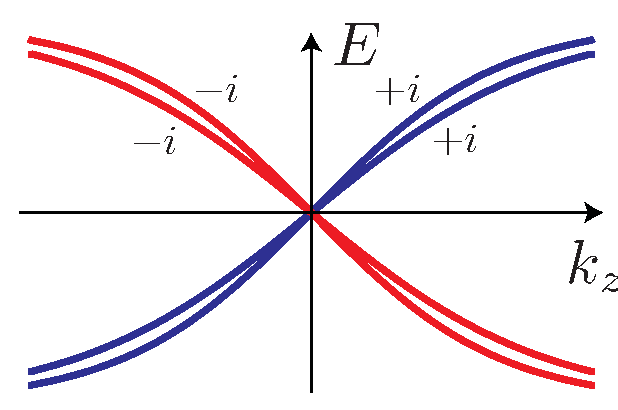
\includegraphics[width=0.25\textwidth]{Diracbands}
\caption{The two pairs of counter-propagating Dirac bands along the $k_z$-axis distinguished by eigenvalues of $C_2=\pm i$.}\label{fig:Diracbands}
\end{figure}

Normally the masslessness of the Dirac system is protected by a set of symmetries. Here, we assume the time reversal (TR) $\mathcal{T}$, which is represented in the single-body picture by the spinful operator $\hat{T}=is_y\mathcal{K}$ where $\mathcal{K}$ is the complex conjugation operator, and a twofold rotation $C_2$ about the $z$-axis. In the case when $\mu_z$ has a non-local origin such as sublattice or orbital, it can enter the rotation operator. We assume $\mathcal{C}_2$ is represented in the single-body picture by $\hat{C}_2=is_z\mu_z$. It squares to minus one in agreement with the fermionic statistics, and commutes with the local time reversal operator. In momentum space, $\mathcal{T}$ flips ${\bf k}\to-{\bf k}$ while $C_2$ rotates $(k_x,k_y,k_z)\to(-k_x,-k_y,k_z)$. The band Hamiltonian \eqref{DiracHam0} shares simultaneous eigenstates with $C_2$ along the $k_z$-axis. The two forward moving bands have $C_2$ eigenvalues $+i$ while the two backward moving ones have $C_2$ eigenvalues $-i$ (see figure~\ref{fig:Diracbands}). Therefore the band crossing is $C_2$-protected while the fourfold degeneracy is pinned at ${\bf k}=0$ because of time reversal symmetry. Noticing that each of the $C_2=\pm i$ sector along the $k_z$-axis is chiral (i.e.~consisting of a single propagating direction), it violates the fermion doubling theorem~\cite{Nielsen_Ninomiya_1981,NielsenNinomiyaPLB1981} and is anomalous. This can be resolved by assuming the $C_2$ symmetry is actually a non-symmorphic screw rotation in the microscopic lattice limit and squares to a primitive lattice translation in $z$. $k_z$ is now periodically defined (up to $2\pi/a$) and the two $C_2$ eigen-sectors wraps onto each other after each period. Focusing on the continuum limit where $k_z$ is small (when compared with $2\pi/a$), $C_2^2=-e^{ik_za}\approx-1$ and the $C_2$ symmetry behaves asymptotically as a proper rotation.

The primary focus of this article is to explore symmetry preserving/enabled interacting topological states that originate from the massless Dirac system. Contrary to its robustness in the single-body non-interacting picture, we show that the 3D Dirac fermion can acquire a many-body mass gap without violating the set of symmetries. To illustrate this, we first make use of the fact that the Dirac system can be turned massive by breaking symmetries. Symmetry breaking inter-valley scatterings introduce two coexisting mass terms \begin{align}H_{\mathrm{Dirac}}({\bf k},{\bf r})=H_{\mathrm{Dirac}}^0({\bf k})+m_x({\bf r})\mu_x+m_y({\bf r})\mu_y\label{DiracHam}\end{align} where $m_x$ (or $m_y$) preserves (resp.~breaks) time reversal, and both of them violate $C_2$. We allow slow spatial modulation of the mass parameters, which can be grouped into a single complex parameter $m({\bf r})=m_x({\bf r})+im_y({\bf r})$, and to be precise, momentum ${\bf k}$ should be taken as a differential operator $-i\nabla_{\bf r}$ when translation symmetry is broken. Non-trivial spatial windings of the symmetry breaking mass parameters give rise to topological line defects or vortices that host protected low-energy electronic degrees of freedom. Proliferation of interacting vortices then provides a theoretical path to multiple massive/massless topological phases while restoring and modifying the original symmetries as they emerge in the low-energy long-length scale effective theory.

\begin{figure}[htbp]
\centering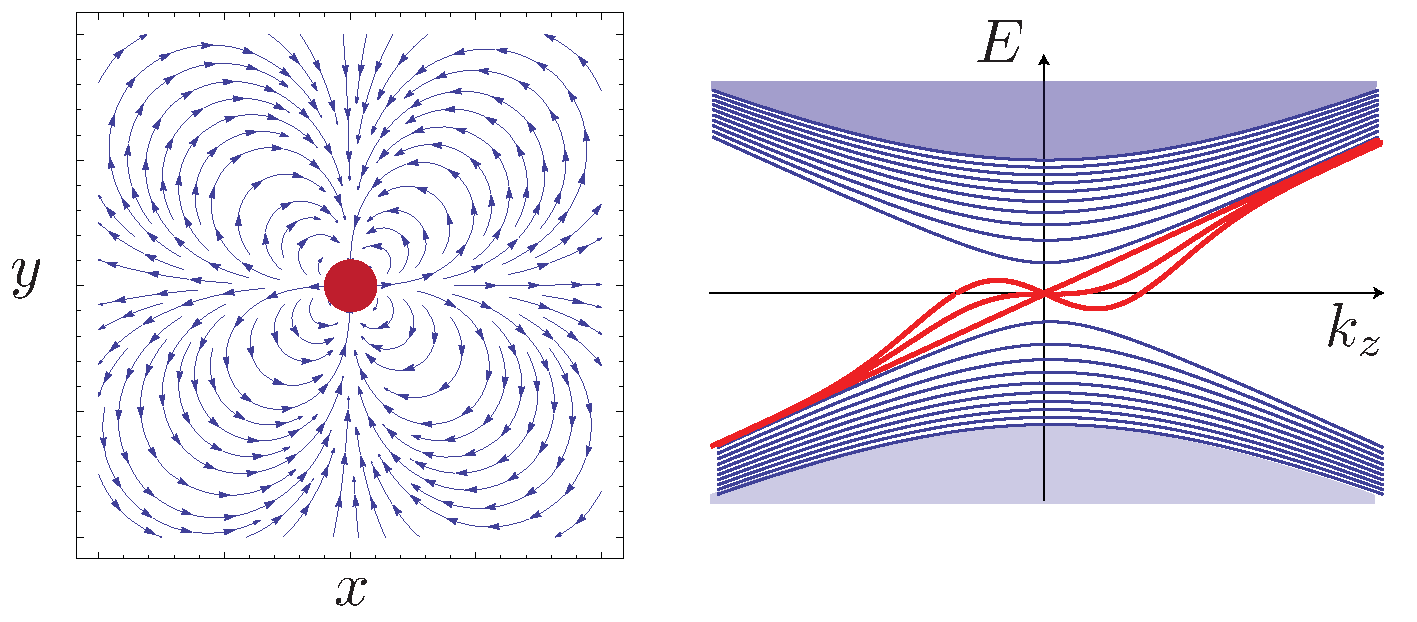
\includegraphics[width=0.4\textwidth]{Diracstring}
\caption{Dirac string. (Left) Spatial winding of mass parameters around a Dirac string going out of the paper represented by the center red dot. Stream lines represent the vector field ${\bf m}({\bf r})=(m_x({\bf r}),m_y({\bf r}))$. (Right) Energy spectrum of chiral Dirac fermions. Blue bands represent bulk continuum. Red bands correspond to chiral Dirac fermions localized along the string.}\label{fig:Diracstring}
\end{figure}

A topological line defect is a vortex string of the mass parameter in three dimensions where the complex phase of $m({\bf r})=|m({\bf r})|e^{i\varphi({\bf r})}$ winds non-trivially around the string. The left diagram in figure~\ref{fig:Diracstring} shows the spatial modulation of $\varphi({\bf r})$ along the $xy$ cross-sectional plane normal to a topological line defect, which runs along the $z$ axis. In this example, the complex phase $\varphi({\bf r})$ winds by $6\pi$ around the line defect (represented by the red dot at the origin). The winding number of the complex phase in general can be evaluated by the line integral \begin{align}c=\frac{1}{2\pi}\oint_\mathcal{C}d\varphi({\bf r})=\frac{1}{2\pi i}\oint_\mathcal{C}\frac{\nabla_{\bf r}m({\bf r})}{m({\bf r})}\cdot d{\bf r}\label{winding}\end{align} where $\mathcal{C}$ is a (righthanded) closed path that runs once around the (oriented) line defect. Eq.\eqref{winding} is always an integer given that the mass parameter $m({\bf r})$ is non-vanishing along $\mathcal{C}$.

Massless chiral Dirac fermions run along these topological line defects~\cite{TeoKane}.

We begin with the Dirac Hamiltonian \eqref{DiracHam} where the mass term winds around a vortex and as a consequence, it hosts a chiral Dirac channel along the vortex (also see figure~\ref{fig:Diracstring}). Here we will demonstrate an example of a simple vortex, and show that there is a chiral Dirac zero mode. In general, the correspondence between the number of protected chiral Dirac channels and the vortex winding is a special case of the Atiyah-Singer Index theorem~\cite{AtiyahSinger63} and falls in the physical classification of topological defects~\cite{TeoKane}.

First, say we start with the Hamiltonian from \eqref{DiracHam}. Then for simplicity we consider the particular Dirac mass $m({\bf r})=m_x({\bf r})+im_y({\bf r})=|m|e^{i\theta}$ that constitute a vortex along the $z$-axis, where $\theta$ is the polar angle on the $xy$-plane. By replacing $k_{x,y}\leftrightarrow-i\partial_{x,y}$, \eqref{DiracHam} becomes \begin{align}H({\bf r})=&\hbar v(-i\partial_xs_x-i\partial_ys_y+k_zs_z)\mu_z\nonumber\\&\;+|m|\cos\theta\mu_x+|m|\sin\theta\mu_y\label{DiracHamapp}\end{align} where $k_z$ is still a good quantum number because translation in $z$ is still preserved. The Hamiltonian can be transformed under a new basis into \begin{align}H'=UHU^{-1}=\left(\begin{smallmatrix}-\hbar vk_z&D\\D^\dagger&\hbar vk_z\end{smallmatrix}\right),\quad U =\left(\begin{smallmatrix}0&1&0&0\\0&0&1&0\\1&0&0&0\\0&0&0&1\end{smallmatrix}\right)\end{align} where the Dirac operator occupying the off-diagonal blocks is \begin{align}D^\dagger &=\left(\begin{smallmatrix}-2i\hbar v\partial_w&|m|e^{-i\theta}\\|m|e^{i\theta}&2i\hbar v \partial_{\bar{w}}\end{smallmatrix}\right)\nonumber\\&=e^{-i\theta\sigma_z}\left(\begin{smallmatrix}-i\hbar v(\partial_r-i \partial_\theta/r)&|m|\\|m|&i\hbar v(\partial_r+i\partial_\theta/r)\end{smallmatrix}\right)\end{align} where $w=x+iy=re^{i\theta}$ and $\sigma_z=\mathrm{diag}(1,-1)$. 

Now we separate the Hamiltonian \begin{align}H'(k_z)=\hbar vk_z\Gamma_5+\left(\begin{smallmatrix}0&D\\D^\dagger&0\end{smallmatrix}\right).\end{align} where $\Gamma_5=\mathrm{diag}(-\openone_2,\openone_2)$. We note that the zero momentum sector $H'(k_z=0)$ has a chiral symmetry since it anticommutes with with $\Gamma_5$, and it reduces to the Jackiw-Rossi vortex problem in two-dimensions~\cite{JackiwRossi81}. The Dirac operator $D^\dagger$ has only one normalizable zero mode $u_0(r)\propto e^{-|m|r/\hbar v}(e^{i\pi/4}, e^{-i\pi/4})^T$, while its conjugate $D$ has none. $H'(k_z=0)$ therefore has a zero eigenvector of $\psi_0(r)=(u_0(r),0)^T$, which is also an eigenvector of $\Gamma_5$. In the full Hamiltonian, the zero mode $\psi_0(r)$ has energy $-\hbar vk_z$ and corresponds a single mid-gap chiral Dirac channel.

When focusing at $k_z=0$, the differential operator \eqref{DiracHam} with a vortex along the $z$-axis is identical to the 2D Jackiw-Rossi model~\cite{JackiwRossi81} with chiral symmetry $\gamma_5=s_z\mu_z$. Each zero energy mode corresponds to a massless chiral Dirac fermion with positive or negative group velocity in $z$ depending on the sign of its $\gamma_5$ eigenvalue. (For a concrete example, see appendix~\ref{sec:chiralmodesapp}) These quasi-one dimensional low-energy electronic modes are similar to those that run along the edge of 2D Landau levels and Chern insulators, except they are now embedded in three dimensions. Their wave functions extend along the defect string direction but are localized and exponentially decay away from the defect line. Moreover, such an electronic channel is chiral in the sense that there is only a single propagating direction. The energy spectrum of the topological line defect (for the example with winding number $c=3$) is shown in the right diagram of figure~\ref{fig:Diracstring}, in which, there are three chiral bands (red curves) inside the bulk energy gap representing the 3 chiral Dirac electrons. As a consequence of the chirality, the transport of charge and energy must also be uni-directional. The chiral electric and energy-thermal responses are respectively captured by the two conductances \begin{align}\sigma=\frac{\delta I_{\mathrm{electric}}}{\delta V}=\nu\frac{e^2}{h},\quad\kappa=\frac{\delta I_{\mathrm{energy}}}{\delta T}=c\frac{\pi^2k_B^2}{3h}T\label{conductance}\end{align} where $\nu$ is the filling fraction if the chiral channel is supported by a 2D insulating bulk, and $c$ is called the chiral central charge. For the Dirac case, $c=\nu$ is the number of chiral Dirac channels. Here $c$ can be negative when the Dirac fermions oppose the preferred orientation of the topological line defect. In a more general situation, $c=c_R-c_L$ counts the difference between the number of forward propagating and backward propagating Dirac fermions. There is a mathematical index theorem~\cite{TeoKane,AtiyahSinger63,Nakaharabook} that identifies the topological winding number in \eqref{winding} and the analytic number of chiral Dirac fermions in \eqref{conductance}. Hence, there is no need to distinguish the two $c$'s. 

The massless chiral Dirac channels, described by the low-energy effective theory \begin{align}\mathcal{L}_{\mathrm{Dirac}}=i\sum_{a=1}^{c_R}\psi^\dagger_a(\partial_t+\tilde{v}\partial_x)\psi_a+i\sum_{b=c_R+1}^{c_R+c_L}\psi^\dagger_b(\partial_t-\tilde{v}\partial_x)\psi_b,\end{align} have an emergent conformal symmetry and the index $c=c_R-c_L$ is also the chiral central charge of the effective conformal field theory (\hypertarget{CFT}{CFT}). We refer to the primitive topological line defect with $c=\pm1$ that hosts one and only chiral Dirac fermion $\psi$ as a {\em Dirac string}. (It should not be confused with the Dirac magnetic flux string that connects monopoles.)

\begin{figure}[htbp]
\centering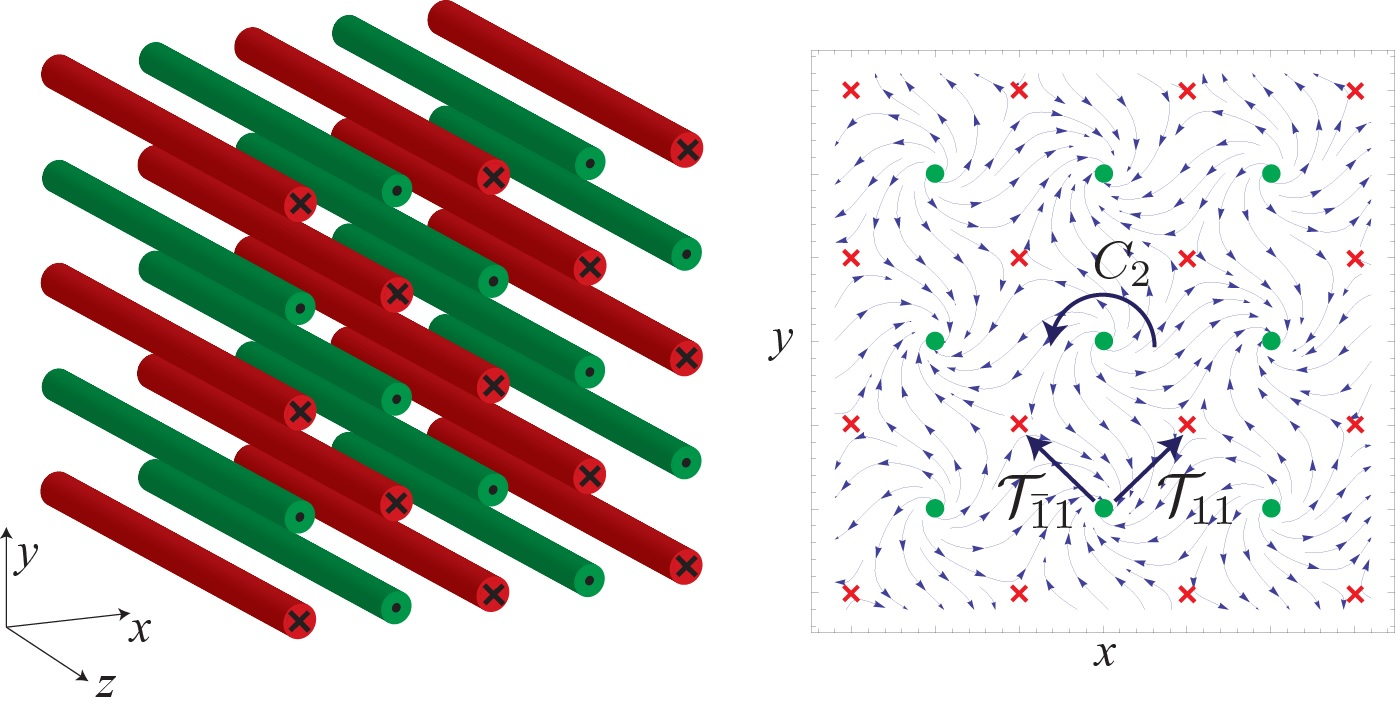
\includegraphics[width=0.45\textwidth]{vortexlattice.jpg}
\caption{(Left) A 3D array of Dirac strings. (Right) Cross section of the array. {\color{red}$\boldsymbol\times$} associates into-the-plane Dirac channel, {\color{green}$\bullet$} represents out-of-plane ones. Stream lines represent the configuration of the mass parameter vector field ${\bf m}({\bf r})=(m_x({\bf r}),m_y({\bf r}))$ of the vortex lattice.}\label{fig:vortexlattice}
\centering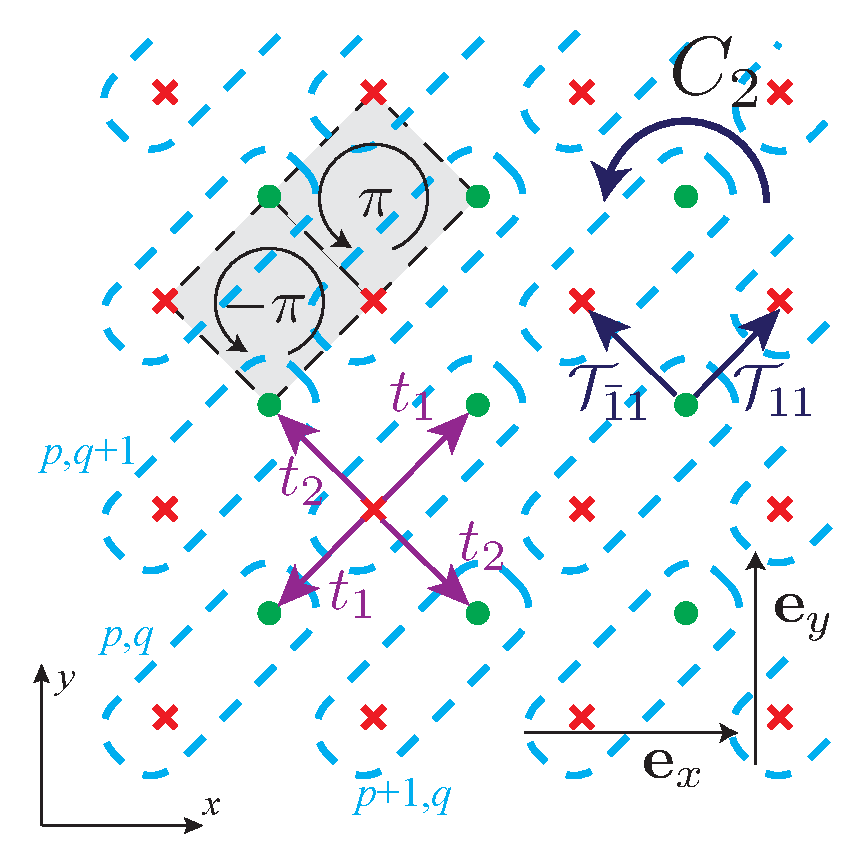
\includegraphics[width=0.25\textwidth]{WeylTB}
\caption{Coupled Dirac wire model with tunneling amplitudes $t_1,t_2$. Each unit cell (dashed box) consists a pair of counter-propagating Dirac strings, {\color{red}$\boldsymbol\times$} and {\color{green}$\bullet$}. $\mathcal{T}_{11},\mathcal{T}_{\bar{1}1}$ are the two anti-ferromagnetic directions.}\label{fig:WeylTB}
\end{figure}

A three-dimensional array of Dirac strings (wires) can be realized as a vortex lattice of the mass parameter $m=m_x+im_y$ in a Dirac semimetal. For example, figure~\ref{fig:vortexlattice} shows a vortex lattice generated by the spatially-varying Dirac mass \begin{align}m({\bf r})=m_0\frac{\mathrm{sd}(x+iy)}{|\mathrm{sd}(x+iy)|},\label{Jacobielliptic}\end{align} where $\mathrm{sd}$ is the (rescaled) Jacobian elliptic function~\cite{ReinhardtWalker10} with simple zeros at $p+iq$ and poles at $(p+1/2)+i(q+1/2)$ for $p,q$ integers. It consists of vortices with alternating winding number $c=\pm1$ at the zeros and poles in a checkered board lattice configuration. On the cross section plot on the right side of figure~\ref{fig:vortexlattice}, there is a Dirac string with positive (or negative) winding at each {\color{green}$\bullet$} (resp. {\color{red}$\boldsymbol\times$}). Each vortex string has a chiral Dirac fermion running through it. Figure~\ref{fig:WeylTB} shows the same two-dimensional slice of the array, except suppressing the mass parameters which correspond to irrelevant microscopic high-energy degrees of freedom. We choose a unit cell labeled by $(p,q)$, its $x,y$ coordinates. Each has both a forward moving Dirac fermion $\psi_{p,q}^\odot$ (shown as {\color{green}$\bullet$}) and a backward moving one $\psi_{p,q}^\otimes$ (shown as {\color{red}$\boldsymbol\times$}). 

This array configuration breaks time reversal as the symmetry would have reversed the chirality (i.e.~propagating direction) of each Dirac fermion. Instead, it has an emergent {\em anti-ferromagnetic time reversal} (AFTR) symmetry, which is generated by the operators $\mathcal{T}_{11}$ and $\mathcal{T}_{\bar{1}1}$ in the diagonal and off-diagonal directions. Each is composed of a time reversal operation and a half-translation by $({\bf e}_x+{\bf e}_y)/2$ or $(-{\bf e}_x+{\bf e}_y)/2$. \begin{gather}\mathcal{T}_{11}\psi_{p,q}^\otimes\mathcal{T}_{11}^{-1}=\psi_{p,q}^\odot,\quad\mathcal{T}_{11}\psi_{p,q}^\odot\mathcal{T}_{11}^{-1}=-\psi_{p+1,q+1}^\otimes\nonumber\\\mathcal{T}_{\bar{1}1}\psi_{p,q}^\otimes\mathcal{T}_{\bar{1}1}^{-1}=\psi_{p-1,q}^\odot,\quad\mathcal{T}_{\bar{1}1}\psi_{p,q}^\odot\mathcal{T}_{\bar{1}1}^{-1}=-\psi_{p,q+1}^\otimes\label{AFTR}\end{gather} These \AFTR operators are non-local as they come with lattice translation parts. They are anti-unitary in the sense that $\mathcal{T}\alpha\psi\mathcal{T}^{-1}=\alpha^\ast\mathcal{T}\psi\mathcal{T}^{-1}$ and $\langle\mathcal{T}u|\mathcal{T}v\rangle=\langle u|v\rangle^\ast$ because the local time reversal symmetry is anti-unitary. %Normally the local \TR operation for a spinful fermion squares to minus one. However, the non-local nature of the \AFTR symmetry allows us to absorb the sign by a non-local gauge transformation (for example $\psi^{\otimes/\odot}_{p,q}\to(-1)^q\psi^{\otimes/\odot}_{p,q}$) so that no signs appear in \eqref{AFTR}. 
Similar to a spatial non-symmorphic symmetry, the \AFTR symmetries square to the primitive translation operators \begin{align}\mathcal{T}_{11}\mathcal{T}_{\bar{1}1}&=(-1)^F\mbox{translation}({\bf e}_y),\nonumber\\\mathcal{T}_{11}\mathcal{T}_{\bar{1}1}^{-1}&=\mbox{translation}({\bf e}_x),\label{AFTRalg}\end{align} where $(-1)^F$ is the fermion parity operator. Moreover they mutually commute $[\mathcal{T}_{11},\mathcal{T}_{\bar{1}1}]=0$. We notice in passing that the \AFTR symmetry is only an emergent symmetry in the low-energy effective theory. It is not preserved in the microscopic Dirac model \eqref{DiracHam} and is broken by the mass parameter, $m({\bf r})\neq m({\bf r}+({\bf e}_x\pm{\bf e}_y)/2)^\ast$. For instance, the Jacobian elliptic Dirac mass function \eqref{Jacobielliptic} actually has a periodic unit cell twice the size of that of the effective wire model in figure~\ref{fig:WeylTB}. On the other hand, the Dirac mass \eqref{Jacobielliptic} is odd under $C_2$, $m(C_2{\bf r})=-m({\bf r})$. This sign is canceled by the $C_2$ rotations of the Dirac matrices, $\hat{C}_2\mu_{x,y}\hat{C}_2^{-1}=-\mu_{x,y}$, that couple with the Dirac mass in the Hamiltonian \eqref{DiracHam}. Therefore the Dirac wire model in figure~\ref{fig:WeylTB} has a twofold axis along one of the Dirac string, say $\psi^\odot_{0,0}$. The Dirac channel fermions transform unitarily according to \begin{align}\mathcal{C}_2\psi^\odot_{p,q}\mathcal{C}_2^{-1}=i\psi^\odot_{-p,-q},\quad\mathcal{C}_2\psi^\otimes_{p,q}\mathcal{C}_2^{-1}=-i\psi^\otimes_{-p+1,-q+1},\label{C2}\end{align} where the factor of $i$ ensures the fermionic $-1$ twist phase for a $2\pi$ rotation, and the second eqaulity in \eqref{C2} is determined by the first one together with \eqref{AFTR} and the symmetry relations \begin{gather}\mathcal{C}_2\mathcal{T}_{11}=(-1)^F\mathcal{T}_{11}^{-1}\mathcal{C}_2,\quad\mathcal{C}_2\mathcal{T}_{\bar{1}1}=(-1)^F\mathcal{T}_{\bar{1}1}^{-1}\mathcal{C}_2.\label{C2Trelation}\end{gather} Again, in order for the rotation symmetric wire model to be free of anomalies, $C_2$ should really be a screw rotation with respect to some microscopic lattice that has become irrelevant in the low-energy continuum picture. \begin{align}\mathcal{C}_2^2=(-1)^F\mathrm{translation}(a{\bf e}_z)\approx(-1)^F.\label{C2square}\end{align}

When adjacent vortex strings are near each other, their Dirac fermion wave functions overlap and there are finite amplitudes of electron tunneling. We construct a coupled Dirac wire model of nearest-wire single-body backscattering processes with $\pm\pi$ fluxes across each diamond square (figure~\ref{fig:WeylTB}), where the tunneling amplitude $t_1$ (or $t_2$) in the $(11)$ (resp.$(\bar{1}1)$) direction is imaginary (resp.~real). \begin{align}\mathcal{H}=&\sum_{p,q}\hbar\tilde{v}\left({\psi_{p,q}^\odot}^\dagger k_z\psi_{p,q}^\odot-{\psi_{p,q}^\otimes}^\dagger k_z\psi_{p,q}^\otimes\right)\nonumber\\&+it_1\left({\psi_{p,q}^\odot}^\dagger\psi_{p,q}^\otimes-{\psi_{p-1,q-1}^\odot}^\dagger\psi_{p,q}^\otimes\right)+h.c.\label{WeylTBHam}\\&+t_2\left({\psi_{p-1,q}^\odot}^\dagger\psi_{p,q}^\otimes-{\psi_{p,q-1}^\odot}^\dagger\psi_{p,q}^\otimes\right)+h.c.\nonumber\end{align} where the first line is the kinetic Hamiltonian of individual Dirac channels under the Fourier transformation $-i\partial_z\leftrightarrow k_z$ along the wire direction. This tight-binding Hamiltonian preserves the \AFTR symmetry \eqref{AFTR}, $\mathcal{T}\mathcal{H}\mathcal{T}^{-1}=\mathcal{H}$. Fourier transformation of the square lattice $\vec\psi_{p,q}=\int\frac{dk_xdk_y}{(2\pi)^2}e^{-i(k_xp+k_yq)}\vec\psi_{\bf k}$, $\vec\psi=(\psi^\odot,\psi^\otimes)$ turns \eqref{WeylTBHam} into $\mathcal{H}=\int\frac{dk_xdk_y}{(2\pi)^2}\vec\psi_{\bf k}^\dagger H(k)\vec\psi_{\bf k}$, where \begin{align}H({\bf k})=\left(\begin{array}{*{20}c}\hbar\tilde{v}k_z&g(k_x,k_y)\\g^\ast(k_x,k_y)&-\hbar\tilde{v}k_z\end{array}\right)\label{BlochHam}\end{align} is the Bloch band Hamiltonian, for $g(k_x,k_y)=it_1(1-e^{-i(k_y+k_x)})+t_2(e^{-ik_x}-e^{-ik_y})$. Here momentum ${\bf k}$ lives in the ``liquid crystal" Brillouin zone (\hypertarget{BZ}{BZ}) where $-\pi\leq k_x,k_y\leq\pi$ and $-\infty<k_z<\infty$ (in the continuum limit $a\to0$ and $\pi/a\to\infty$). 

\begin{figure}[htbp]
\centering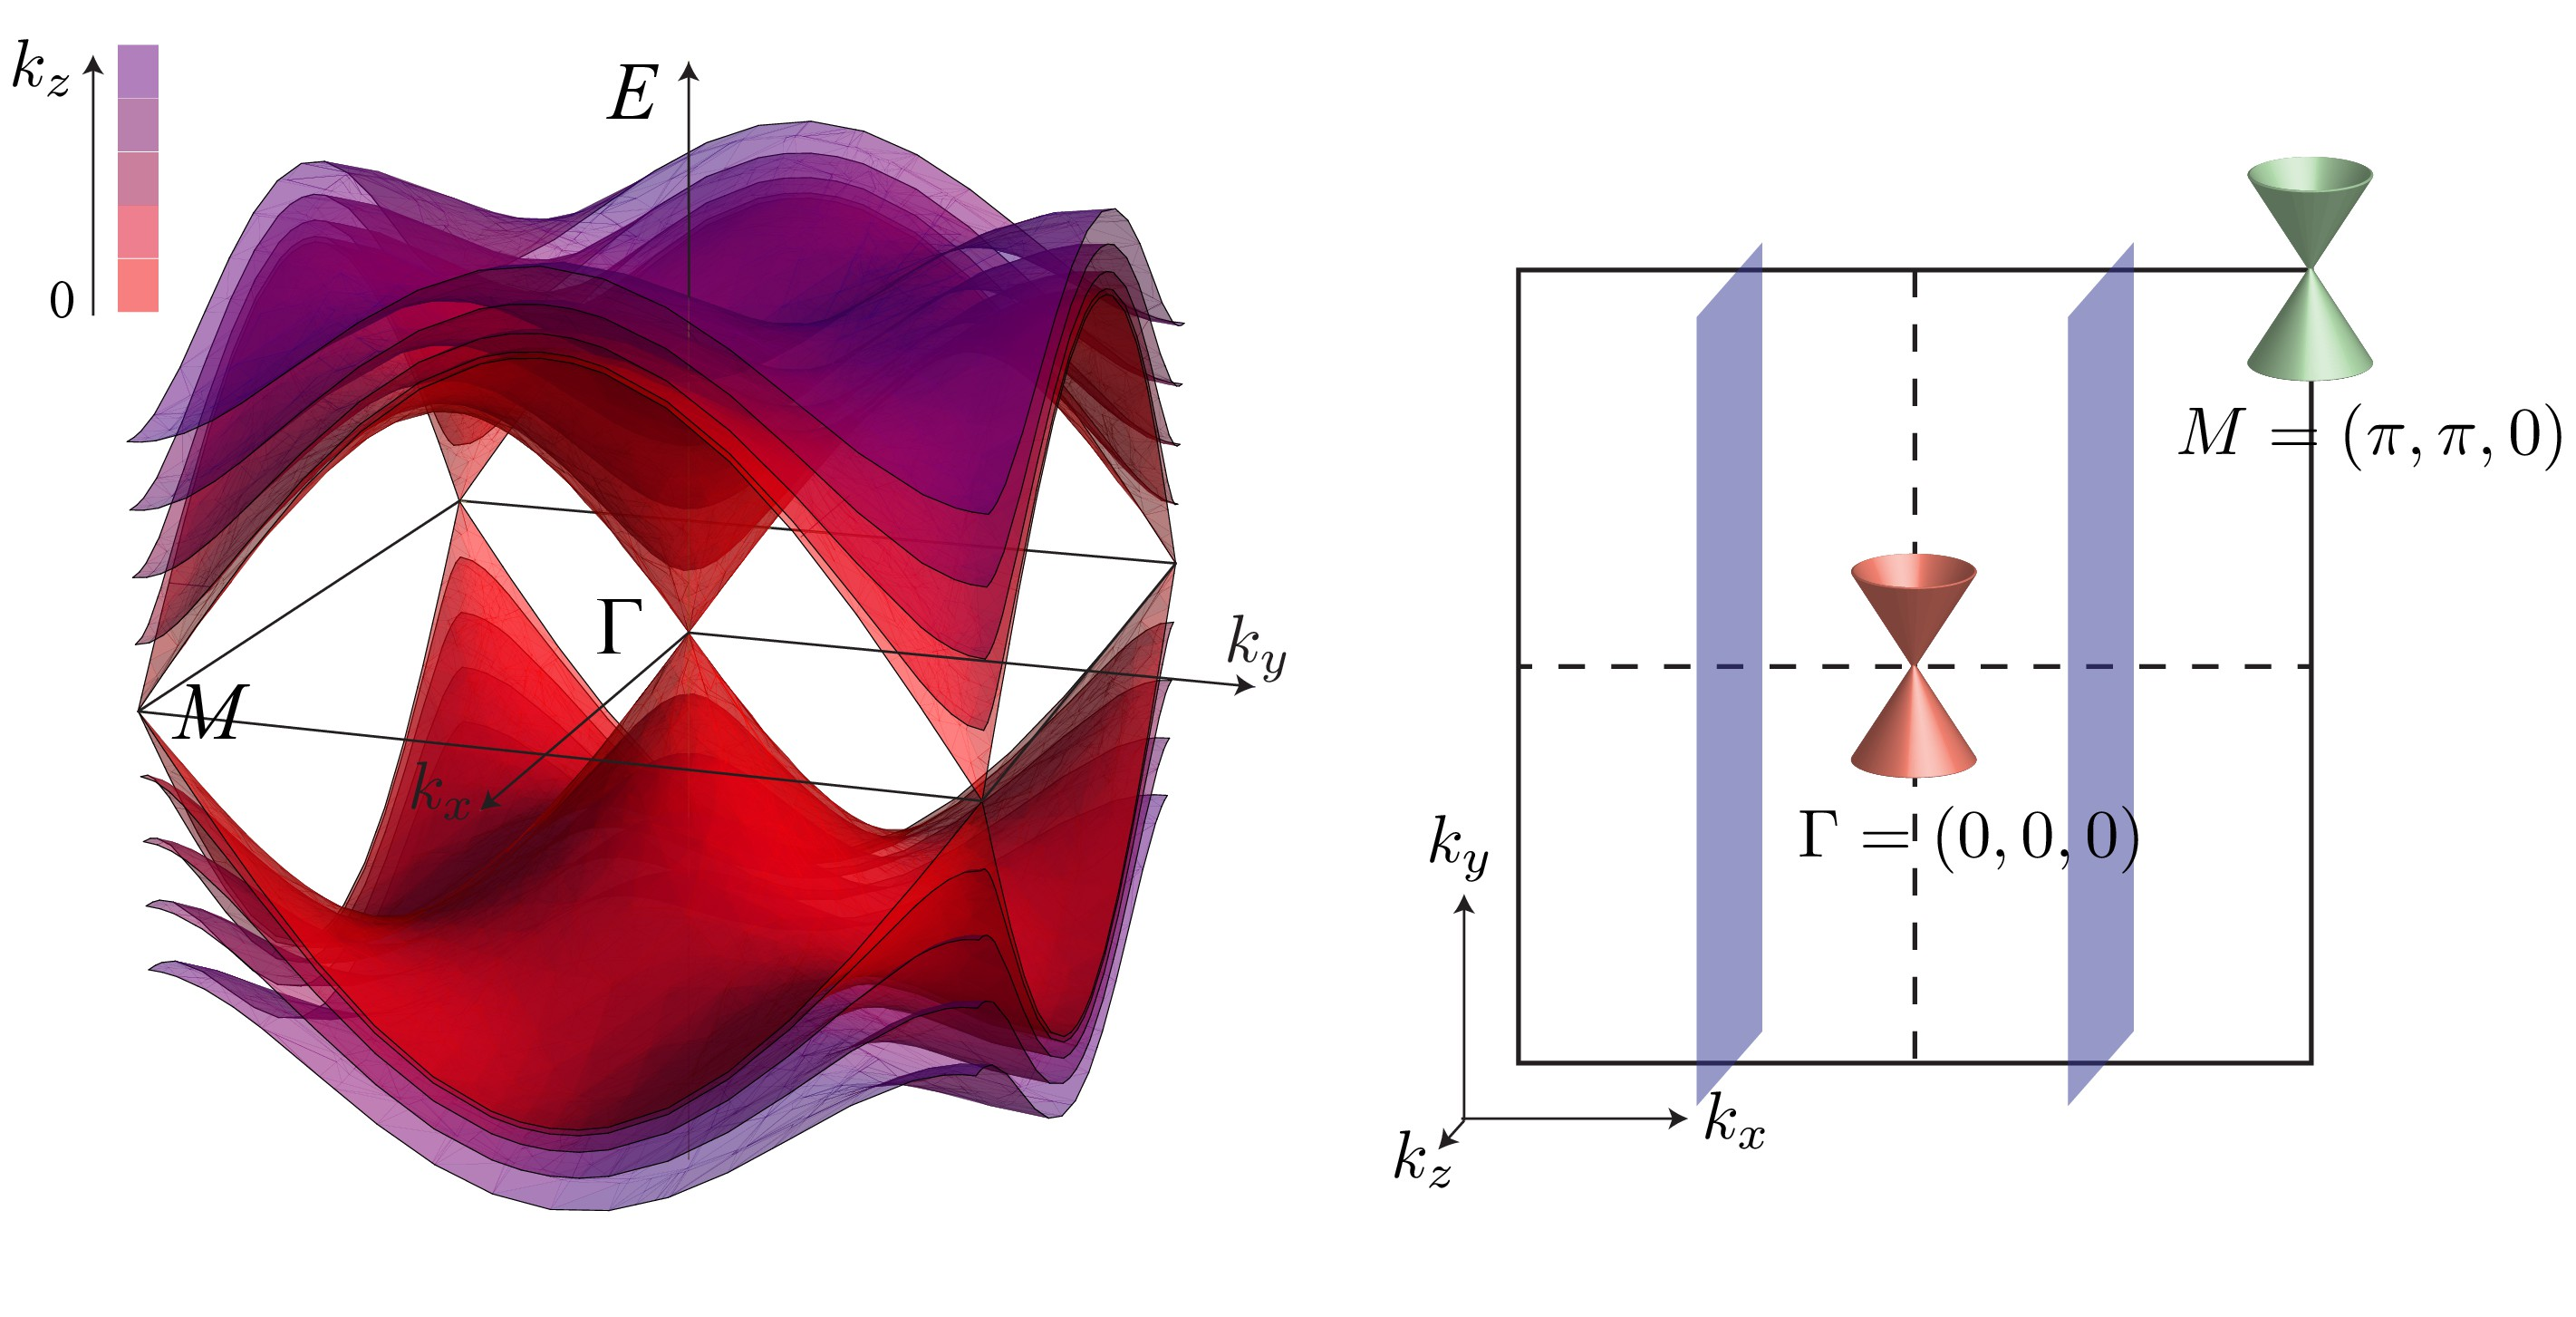
\includegraphics[width=0.45\textwidth]{Weylspectrumjpg.jpg}
\caption{Energy spectrum of the coupled Dirac wire model \eqref{WeylTBHam}.}\label{fig:Weylspectrum}
\end{figure}

The energy spectrum of the two-band model is given by $E_\pm({\bf k})=\pm\sqrt{|g(k_x,k_y)|^2+\hbar^2\tilde{v}^2k_z^2}$ (see figure~\ref{fig:Weylspectrum}).
It gives two linearly dispersing Weyl cones of opposite chiralities in the Brillouin zone centered at $K^+_0=\Gamma=(0,0,0)$ and $K^-_0=M=(\pi,\pi,0)$. Near these points, the Hamiltonians are of the linear form $H(K_0^\pm+\delta{\bf k})=\hbar\delta{\bf k}^TV^\pm\vec\sigma+O(\delta k^2)$, where $\vec\sigma=(\sigma_x,\sigma_y,\sigma_z)$ are Pauli matrices acting on the $(\psi^\odot,\psi^\otimes)$ degrees of freedom. The velocity matrices are \begin{align}\hbar V^\pm=\left(\begin{array}{ccc}-t_1&\pm t_2&0\\-t_1&\mp t_2&0\\0&0&\hbar\tilde{v}\end{array}\right),\end{align} whose determinant's %$\det(\hbar V)=\pm2\hbar\tilde{v}t_1t_2$ 
sign decides the $\pm$ chirality of the Weyl fermion at $\Gamma$ and $M$, i.e.~the $\pm1$ Fermi surface Chern invariants~\cite{WanVishwanathSavrasovPRB11,Ashvin_Weyl_review,RMP}. %Expanding about the two Weyl points and ignoring higher order terms gives $H(X^{\pm} + \delta {\mathbf{k}})= -t_1 (\delta k_x + \delta k_y) \sigma_x  \mp t_2 (\delta k_x - \delta k_y) \sigma_y  + v \delta k_z \sigma_z$.
The \AFTR symmetries \eqref{AFTR} in the single-body picture are expressed under Fourier transformation as \begin{gather}\mathcal{T}_{11}\vec\psi_{\bf k}\mathcal{T}_{11}^{-1}=T_{11}({\bf k})\vec\psi_{-\bf k},\quad\mathcal{T}_{\bar{1}1}\vec\psi_{\bf k}\mathcal{T}_{\bar{1}1}^{-1}=T_{\bar{1}1}({\bf k})\vec\psi_{-\bf k},\nonumber\\T_{11}({\bf k})=\left(\begin{array}{ccc}0&-e^{i(k_x+k_y)}\\1&0\end{array}\right)\mathcal{K},\nonumber\\T_{\bar{1}1}({\bf k})=\left(\begin{array}{ccc}0&-e^{ik_y}\\e^{-ik_x}&0\end{array}\right)\mathcal{K},\label{AFTRk}\end{gather} where $\mathcal{K}$ is the complex conjugation operator. They satisfy the appropriate algebraic relations \eqref{AFTRalg} in momentum space \begin{gather}T_{11}(-{\bf k})T_{\bar{1}1}({\bf k})=T_{\bar{1}1}(-{\bf k})T_{11}({\bf k})=-e^{-ik_y}\nonumber\\T_{11}(-{\bf k})T_{\bar{1}1}({\bf k})^{-1}=T_{\bar{1}1}(-{\bf k})^{-1}T_{11}({\bf k})=e^{-ik_x}\end{gather} and the coupled wire model \eqref{BlochHam} is \AFTR symmetric \begin{align}T_{11}({\bf k})H({\bf k})&=H(-{\bf k})T_{11}({\bf k}),\nonumber\\T_{\bar{1}1}({\bf k})H({\bf k})&=H(-{\bf k})T_{\bar{1}1}({\bf k}).\label{WeylTBT11}\end{align} The Weyl points are at time reversal invariant momenta (\hypertarget{TRIM}{TRIM}) $K^\pm_0\equiv-K^\pm_0$ (modulo the reciprocal lattice $2\pi\mathbb{Z}^2$), and the \AFTR operators $T_{11}(K^\pm_0)=-i\sigma_y\mathcal{K}$ and $T_{\bar{1}1}(K^\pm_0)=\mp i\sigma_y\mathcal{K}$ square to minus one. Hence the Weyl points are not only protected by the non-vanishing Fermi surface Chern invariant but also the Kramers' theorem. In addition, the model is also $C_2$ symmetric \begin{align}C_2({\bf k})H({\bf k})=H(C_2{\bf k})C_2({\bf k})\label{WeylTBC2}\end{align} where the twofold symmetry \eqref{C2} is represented in the single-body picture by a diagonal matrix \begin{align}\mathcal{C}_2\vec\psi_{\bf k}\mathcal{C}_2^{-1}=C_2({\bf k})\vec\psi_{\bf k},\quad C_2({\bf k})=\left(\begin{array}{*{20}c}i&0\\0&-ie^{-i(k_x+k_y)}\end{array}\right)\label{C2k}\end{align} (supressing the screw phase $e^{-ik_za/2}$ in the continuum limit $a\to0$). It agrees with the fermion statistics \eqref{C2square} $C_2(-k_x,-k_y,k_z)C_2(k_x,k_y,k_z)=-1$, and the algebraic relations \eqref{C2Trelation} with the \AFTR operators \begin{align}C_2(-{\bf k})T_{11}({\bf k})&=-T_{11}(C_2{\bf k})^{-1}C_2({\bf k})\nonumber\\C_2(-{\bf k})T_{\bar{1}1}({\bf k})&=-T_{\bar{1}1}(C_2{\bf k})^{-1}C_2({\bf k})\end{align} for $C_2{\bf k}=(-k_x,-k_y,k_z)$.

\subsubsection{The anomalous Dirac semimetal}\label{sec:anomaly}
We notice that the coupled wire Dirac model \eqref{WeylTBHam} and its massless energy spectrum in figure~\ref{fig:Weylspectrum} are anomalous with respect to the \AFTR symmetries $\mathcal{T}_{11}$ and $\mathcal{T}_{\bar{1}1}$ as well as the $C_2$ symmetry if it is proper symmorphic and not a screw rotation. This means that it cannot be realized in a single-body three dimensional lattice system with the \AFTR or $C_2$ symmetries. In a sense, it is not surprising at all since the chiral Dirac strings that constitute \eqref{WeylTBHam} are themselves violating fermion doubling~\cite{Nielsen_Ninomiya_1981,NielsenNinomiyaPLB1981}. Here we further elaborate on the anomalous Dirac spectrum (figure~\ref{fig:Weylspectrum}) where the pair of Weyl points are separately located at two time reversal invariant momenta $K^\pm_0$. We also comment on the non-trivial consequence of the anomaly and pave the path for later discussion on many-body interactions.

We begin with two 2D planes in momentum space parallel to $k_yk_z$ located at $k_x=\pm\pi/2$. They are represented by the two blue planes in figure~\ref{fig:Weylspectrum}. The \AFTR or $C_2$ symmetries require the Chern invariants \begin{align}\mathrm{Ch}_1=\frac{i}{2\pi}\int\mathrm{Tr}(P\partial_{k_y}P\partial_{k_z}P)dk_ydk_z\label{1stChern}\end{align} at $k_x=\pm\pi/2$ to be opposite, where $P({\bf k})=(\openone-H({\bf k})/|E({\bf k})|)/2$ is the projection operator onto the negative energy band. This is because the \AFTR symmetry is anti-unitary and preserves the orientation of the $k_yk_z$ plane, whereas $C_2$ is unitary but reverses the orientation of the $k_yk_z$ plane. Here we present a proof. 

We begin with a Bloch Hamiltonian $H({\bf k})$ that is symmetric under the operation $G({\bf k})$, \begin{align}H({\bf k})&=G(g{\bf k})H(g{\bf k})G(g{\bf k})^{-1}\end{align} if $G$ is unitary, or \begin{align}H({\bf k})&=G(g{\bf k})H(g{\bf k})^\ast G(g{\bf k})^{-1}\end{align} if it is antiunitary. Let $|u_m({\bf k})\rangle$ be the occupied states of $H({\bf k})$. We define $|u'_m({\bf k})\rangle=|Gu_m({\bf k})\rangle=G(g{\bf k})|u_m(g{\bf k})\rangle$ (or $|u'_m({\bf k})\rangle=|Gu_m({\bf k})\rangle=G(g{\bf k})|u_m(g{\bf k})^\ast\rangle$), which is also an occupied state of $H({\bf k})$, for unitary (resp.~antiunitary) symmetry.

The Chern number \eqref{1stChern} can equivalently be defined as \begin{align}\mathrm{Ch}_1(k_x)=\frac{i}{2\pi}\int_{\mathcal{N}_{k_x}}\mathrm{Tr}\left(\mathcal{F}_{\bf k}\right)\label{1stChernapp}\end{align} where $\mathrm{Tr}\left(\mathcal{F}_{\bf k}\right)=d\mathrm{Tr}\left(\mathcal{A}_k\right)$, $\mathcal{N}_{k_x}$ is the oriented $k_yk_z$-plane with fixed $k_x$, and $\mathcal{A}_k$ is the Berry connection of the occupied states $\mathcal{A}_{\bf k}^{mn}=\langle u_m({\bf k})|du_n({\bf k})\rangle$. The Berry connection transforms according to \begin{align}{\mathcal{A}'}_{\bf k}^{mn}&\equiv\langle u'_m({\bf k})|du'_n({\bf k})\rangle\\&=\langle u_m(g{\bf k})|G(g{\bf k})^\dagger d \left[G(g{\bf k})|u_n(g{\bf k})\rangle\right]\nonumber\\&=\mathcal{A}_{g{\bf k}}^{mn}+\langle u_m(g{\bf k})|\left[G(g {\bf k})^\dagger dG(g {\bf k})\right]|u_n(g{\bf k})\rangle\nonumber\end{align} for unitary $G$, or \begin{align}{\mathcal{A}'}_{\bf k}^{mn}&=\left(\mathcal{A}_{g{\bf k}}^{mn}\right)^\ast+\langle u_m(g{\bf k})^\ast|\left[G(g {\bf k})^\dagger dG(g {\bf k})\right]|u_n(g{\bf k})^\ast\rangle\nonumber\\&=-\mathcal{A}_{g{\bf k}}^{nm}+\langle u_m(g{\bf k})^\ast|\left[G(g {\bf k})^\dagger dG(g {\bf k})\right]|u_n(g{\bf k})^\ast\rangle\nonumber\end{align} if $G$ is antiunitary, because the connection is skew-hermitian $\mathcal{A}=-\mathcal{A}^\dagger$. Therefore \begin{align}%\mathrm{Tr}(\mathcal{A}'_{\bf k})&=\mathrm{Tr}(\mathcal{A}_{g{\bf k}})+\mathrm{Tr}\left\{P_{g \bf{k}}\wedge\left[G(g{\bf k})^\dagger dG(g {\bf k})\right]\right\},\nonumber\\
\mathcal{F}'_{\bf k}&=\mathcal{F}_{g{\bf k}}+d\mathrm{Tr}\left\{P_{g\bf{k}}\wedge\left(G(g{\bf k})^\dagger dG(g{\bf k})\right]\right\}\label{curvature}\end{align} for an unitary symmetry, or \begin{align}%\mathrm{Tr}(\mathcal{A}'_{\bf k})&=-\mathrm{Tr}(\mathcal{A}_{g{\bf k}})+\mathrm{Tr}\left\{P_{g \bf{k}}^\ast\wedge\left[G(g{\bf k})^\dagger dG(g {\bf k})\right]\right\},\nonumber\\
\mathcal{F}'_{\bf k}&=-\mathcal{F}_{g{\bf k}}+d\mathrm{Tr}\left\{P_{g\bf{k}}^\ast\wedge\left(G(g{\bf k})^\dagger dG(g{\bf k})\right]\right\}\label{curvature2}\end{align} for an antiunitary one. Here $P({\bf k})=\sum_n|u_n({\bf k})\rangle\langle u_n({\bf k})|$ is the projection operator on to the occupied energy states at momentum ${\bf k}$. Since the trace of Berry curvature $\mathrm{Tr}(\mathcal{F})$ does not depend on the gauge choice of occupied states, $\mathrm{Tr}(\mathcal{F}_{\bf k})=\mathrm{Tr}(\mathcal{F}'_{\bf k})$. We notice the final terms in both \eqref{curvature} and \eqref{curvature2} integrate to zero over the closed periodic momentum plane $\mathcal{N}_{k_x}$. This is because they are total derivatives, and unlike $\mathcal{A}_{\bf k}$, $P_{\bf k}$ and $G({\bf k})$ are defined non-singularly on the entire Brillouin zone (see \eqref{AFTRk} and \eqref{C2k}). 

Now we derive the relation between the Chern number \eqref{1stChernapp} between $k_x$ and $-k_x$ using the antiunitary \AFTR and the unitary $\mathcal{C}_2$ symmetries. The \AFTR symmetries flip all momentum axes $\mathcal{T}_{11},\mathcal{T}_{\bar{1}1}:(k_x,k_y,k_z)\mapsto(-k_x,-k_y,-k_z)$, while the $\mathcal{C}_2$ symmetry flips only two $\mathcal{C}_2:(k_x,k_y,k_z)\mapsto(-k_x,-k_y,k_z)$. Thus, $\mathcal{T}_{11},\mathcal{T}_{\bar{1}1}:\mathcal{N}_{k_x}\to\mathcal{N}_{-k_x}$ maps between opposite planes while preserving their orientations, but $\mathcal{C}_2:\mathcal{N}_{k_x}\to-\mathcal{N}_{-k_x}$ is orientation reversing. Lastly, we substitute \eqref{curvature} and \eqref{curvature2} into \eqref{1stChernapp}, and apply a change of integration variable ${\bf k}\leftrightarrow g{\bf k}$. The \AFTR and $\mathcal{C}_2$ requires the Chern number to flip under $k_x\leftrightarrow-k_x$ \begin{align}\mathrm{Ch}_1(k_x)=-\mathrm{Ch}_1(-k_x).\end{align}


 On the other hand, the two Chern invariants along the two planes must differ by 1 because they sandwich a single Weyl point at $\Gamma$. This forces the Chern invariants to be a half integer $\mathrm{Ch}_1=\pm1/2$, which is anomalous.

While the $C_2$ anomaly can be resolved simply by doubling the unit cell and assuming it originates from a microscopic non-symmorphic screw axis, the \AFTR anomaly is stronger because the two antiferromagnetic combinations \eqref{AFTRalg} generate lattice translations and fix the unit cell size. There are three resolutions. \begin{enumerate}\item The \AFTR symmetries are broken by high energy degrees of freedom when $k_z$ is large. \item The spectrum in figure~\ref{fig:Weylspectrum} is the holographic 3D boundary spectrum of an \AFTR symmetric weak topological insulator in 4D. \item The spectrum is generated by strong many-body interaction non-holographically in 3D.\end{enumerate} Below we discuss the first two resolutions, and we leave the many-body interaction-enabled situation to section~\ref{sec:intenable}.

\subsubsection{Broken symmetries and coarse-graining}\label{sec:brokensymmetry}
In the present case when the chiral Dirac channels originate from vortex strings in an underlying microscopic Dirac insulator, the spatial modulation of mass parameters $m({\bf r})$ actually violate one of the \AFTR symmetries, $m({\bf r})^\ast\neq m({\bf r}+({\bf e}_x\pm{\bf e}_y)/2)$, where $\ast$ stands for complex conjugation. For instance, since all elliptic functions must contain at least two zeros and two poles in its periodic cell, the Jacobian elliptic mass function \eqref{Jacobielliptic} has longer periods than ${\bf e}_x$ and ${\bf e}_y$ in figure~\ref{fig:WeylTB}, and thus must break $\mathcal{T}_{11}$ or $\mathcal{T}_{\bar{1}1}$. The symmetry is broken only in the ultra-violet limit at large $k_z$ where the chiral Dirac line nodes meet the microscopic bulk band (see figure~\ref{fig:Diracstring}) at high energy $\sim|m({\bf r})|$. In fact, the above anomalous argument shows that {\em all} mass parameter configurations that produce the 3D vortex lattice array (figure~\ref{fig:vortexlattice}) must either (a) break both the \AFTR symmetries $\mathcal{T}_{11}$ and $\mathcal{T}_{\bar{1}1}$, or (b) preserve one but violate translation so that the unit cell is enlarged and the two Weyl points collapse onto each other in momentum space. (See figure~\ref{fig:Chernstack} and \ref{fig:DiracTB}.)

For instance, the microscopic system can be connected to a stack of Chern insulating ribbons (or lowest Landau levels) with alternating chiralities shown in figure~\ref{fig:Chernstack}. Instead of being supported by vortices of Dirac mass, the chiral Dirac wires are now realized as edge modes of Chern insulating strips. Each 2D ribbon (represented by thick dashed dark blue lines) is elongated in the out-of-paper $z$-direction but is finite along the $(110)$ direction and holds counter-propagating boundary chiral Dirac channels. The dark blue arrows represent the orientations of the Chern ribbons that accommodate the boundary Dirac channels with the appropriate propagating directions. Here the Chern ribbon pattern in figure~\ref{fig:Chernstack}(a) breaks both \AFTR axes. The pattern in figure~\ref{fig:Chernstack}(b) preserves $\mathcal{T}_{\bar{1}1}$. However, translation symmetry is also broken and the coupled Dirac wire model now has an enlarged unit cell (light blue dashed boxes) that consists of two pairs of counter-propagating chiral Dirac channels. All Chern ribbon patterns must break the $C_2$ symmetry about a Dirac wire because each wire is connected to one and only one Chern ribbon in a particular direction.

\begin{figure}[htbp]
\centering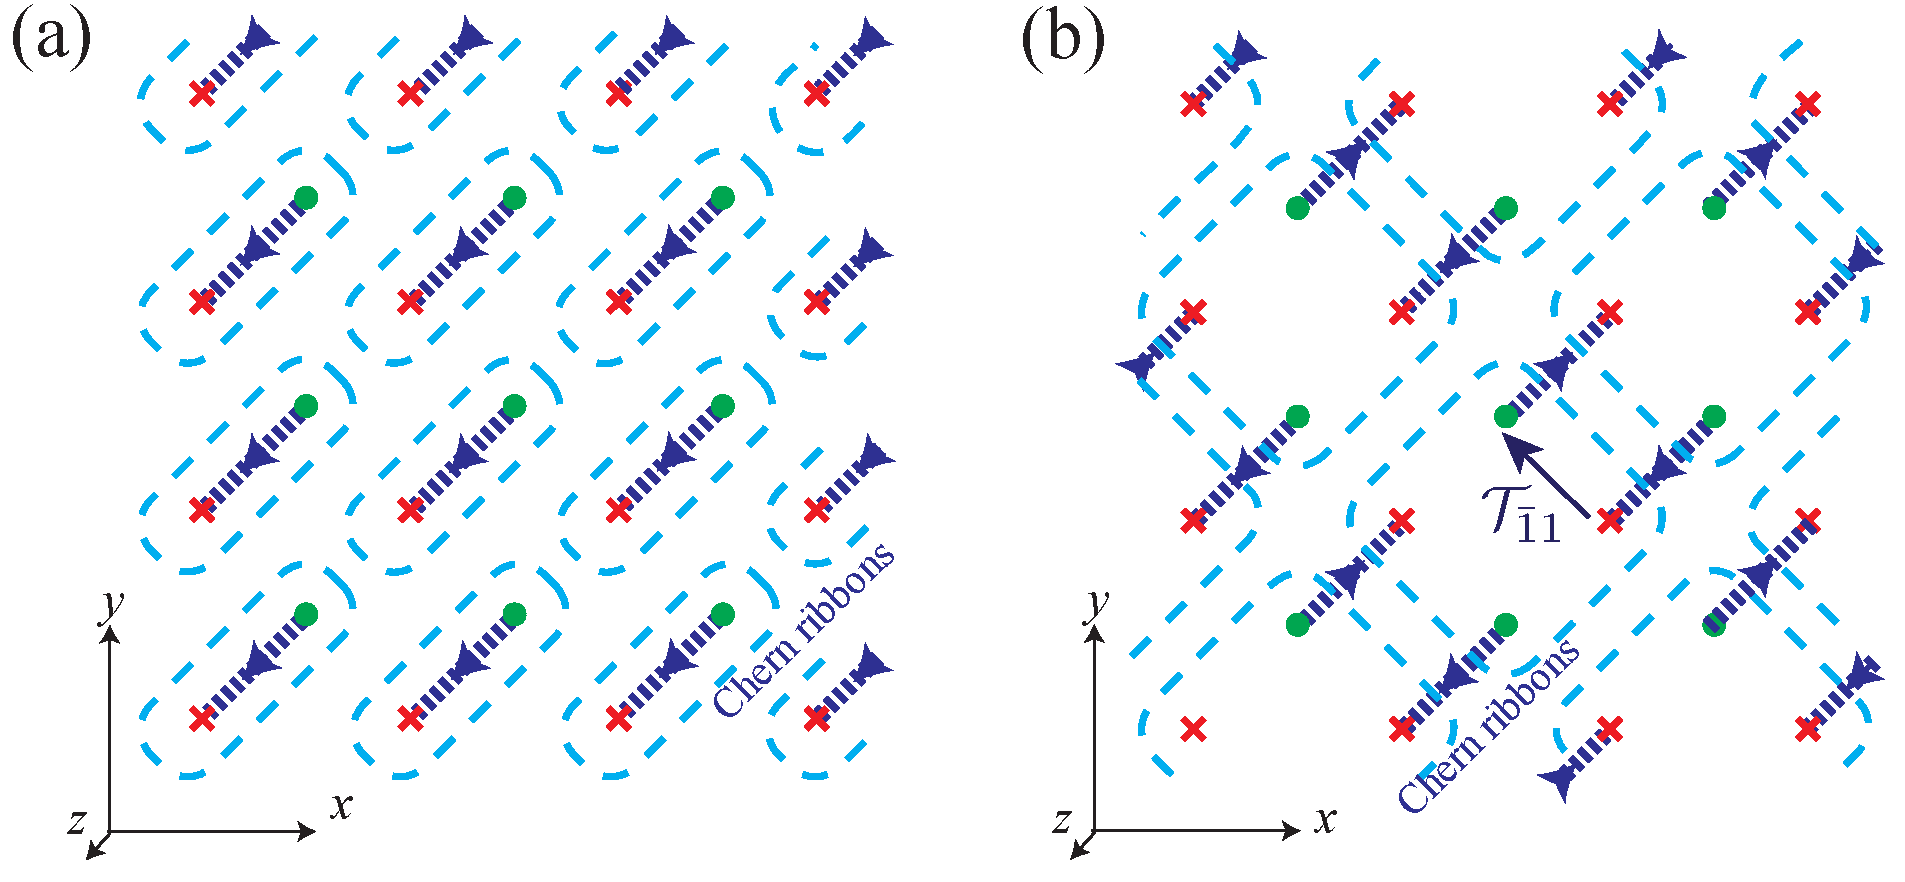
\includegraphics[width=0.45\textwidth]{Chernstack}
\caption{Chiral Dirac channels ({\color{red}$\boldsymbol\times$} and {\color{green}$\bullet$}) realized on the edge of Chern insulating ribbons (dark blue directed lines) stacked along the $(\bar{1}10)$ normal direction.}\label{fig:Chernstack}
\end{figure}

Now we go back to the vortex lattice generated by the Jacobian elliptic Dirac mass function $m({\bf r})$ in \eqref{Jacobielliptic} and consider its symmetries. For this purpose, we use the symmetry properties of the (rescaled) Jacobian elliptic function~\cite{ReinhardtWalker10} \begin{align}&\mathrm{sd}(x+iy)=-\mathrm{sd}(x+1+iy)=-\mathrm{sd}(x+iy+i)\nonumber\\&\mathrm{sd}\left(x+iy+\frac{1+i}{2}\right)=-i\frac{C}{\mathrm{sd}(x+iy)}\label{sdprop}\\&\mathrm{sd}(-x-iy)=-\mathrm{sd}(x+iy)\nonumber\end{align} where $C$ is some unimportant real constant that depends on the modulus of $\mathrm{sd}$ and will never appear in the mass function $m({\bf r})=m_0\mathrm{sd}(x+iy)/|\mathrm{sd}(x+iy)|$. We see from the minus sign in the first equation that the Jacobian elliptic function, and consequently the mass function, have primitive periods ${\bf e}_x\pm{\bf e}_y$ and therefore have a unit cell of size 2 (see figure~\ref{fig:DiracTB}(a)). Choosing $m_0=|m_0|e^{i\pi/4}$, we see from the second equation that $\mathcal{T}_{11}$ (or $\mathcal{T}_{\bar{1}1}$) is preserved (resp.~broken) \begin{align}m\left({\bf r}+\frac{{\bf e}_x\pm{\bf e}_y}{2}\right)=\pm m({\bf r})^\ast,\label{massT11}\end{align} and thus the parent Dirac Hamiltonian \eqref{DiracHam} is $\mathcal{T}_{11}$-symmetric \begin{align}\hat{T}H_{\mathrm{Dirac}}\left(-{\bf k},{\bf r}+\frac{{\bf e}_x+{\bf e}_y}{2}\right)\hat{T}^{-1}=H_{\mathrm{Dirac}}({\bf k},{\bf r}),\end{align} for $\hat{T}=is_y\mathcal{K}$. Lastly, the third property of \eqref{sdprop} entails the mass function $m({\bf r})=-m(C_2{\bf r})$ is odd under $C_2$, and consequently the parent Dirac Hamiltonian is (screw) rotation symmetric \begin{align}\hat{C}_2H_{\mathrm{Dirac}}(C_2{\bf k},C_2{\bf r})\hat{C}_2^{-1}=H_{\mathrm{Dirac}}({\bf k},{\bf r}),\label{massC2}\end{align} where $\hat{C}_2=is_z\mu_z$ (or microscopically $e^{-ik_za/2}is_z\mu_z$) anticommuting with the mass terms $m_1\mu_x+m_2\mu_y$ in $H_{\mathrm{Dirac}}$ (see \eqref{DiracHam}), and $C_2{\bf k}=(-k_x,-k_y,k_z)$, $C_2{\bf r}=(-x,-y,z)$.

\begin{figure}[htbp]
\centering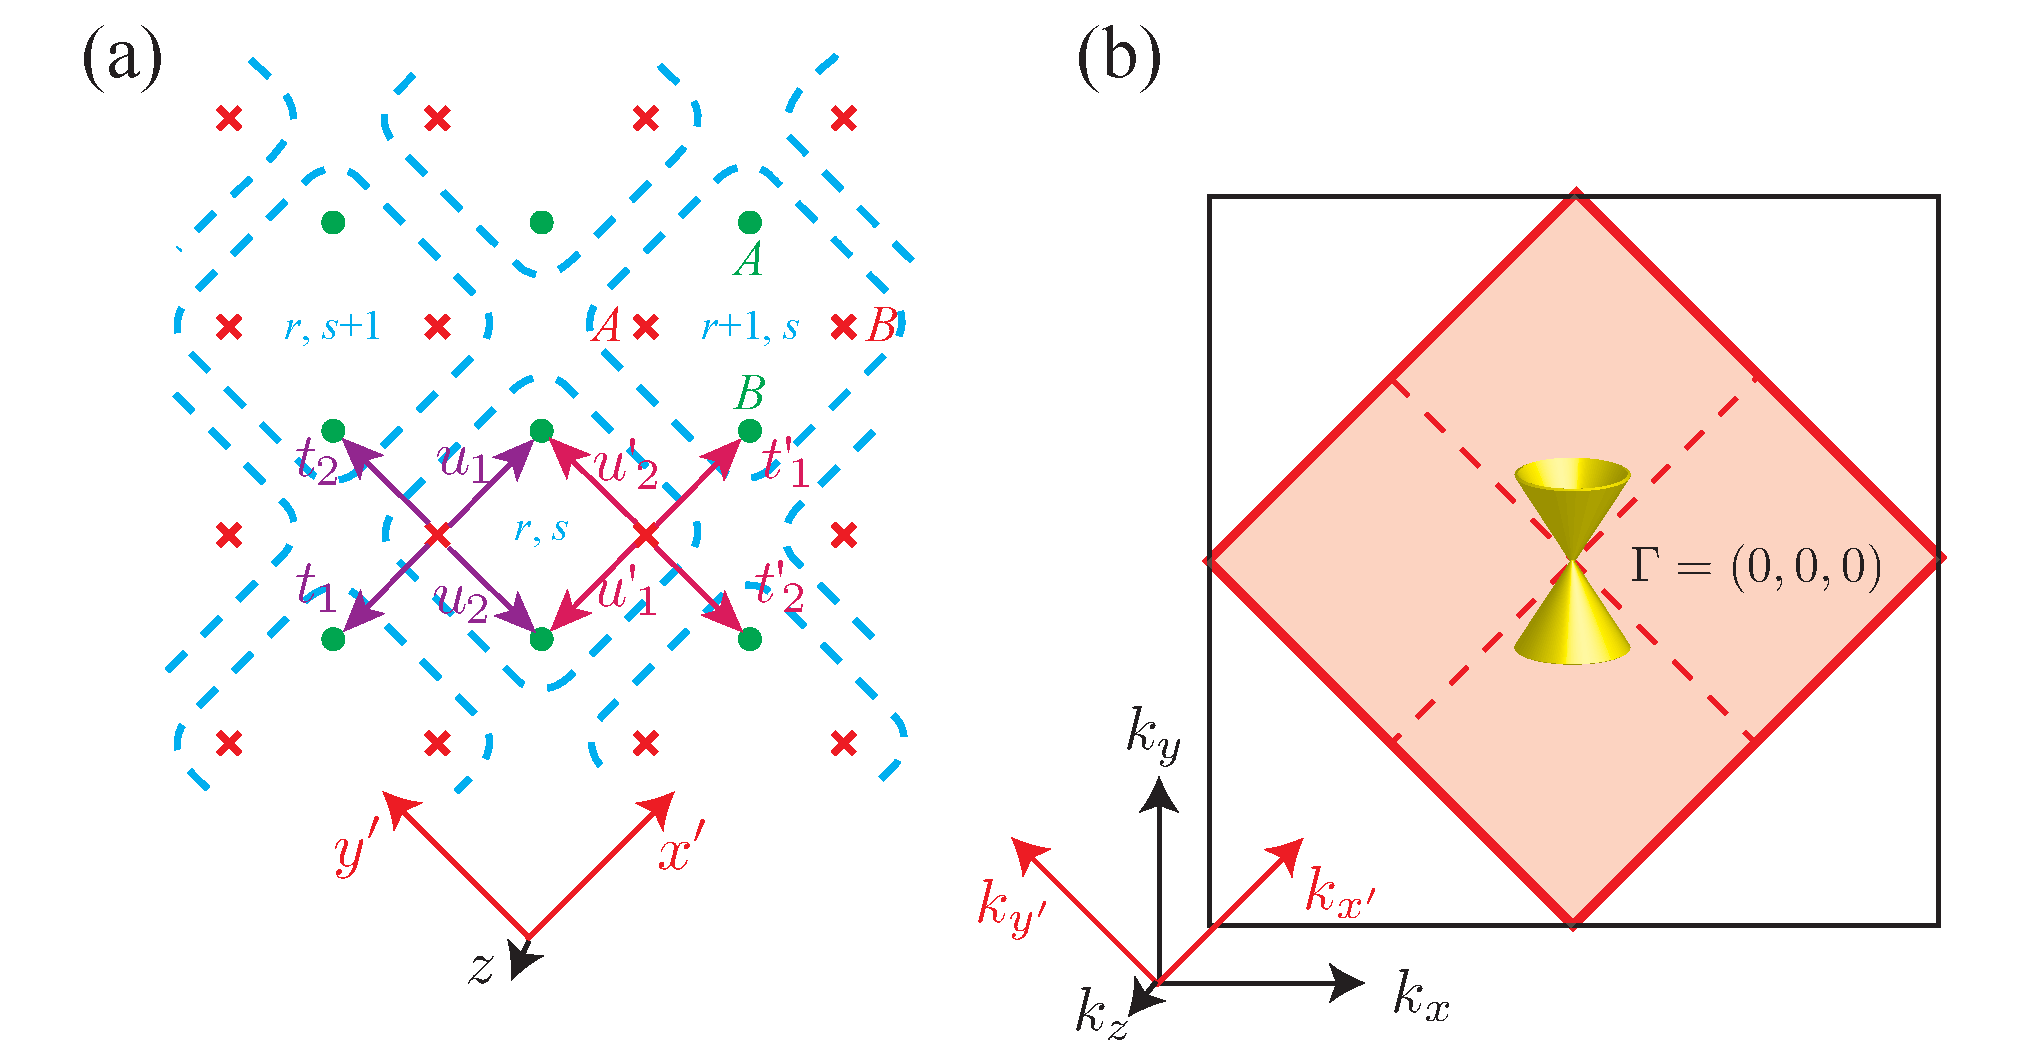
\includegraphics[width=0.45\textwidth]{DiracTB}
\caption{(a) The massive AFTR and $C_2$ breaking coupled Dirac wire model. (b) The reduced Brillouin zone (BZ) after translation symmetry breaking where the two Weyl points collapse to a single Dirac point at $M$.}\label{fig:DiracTB}
\centering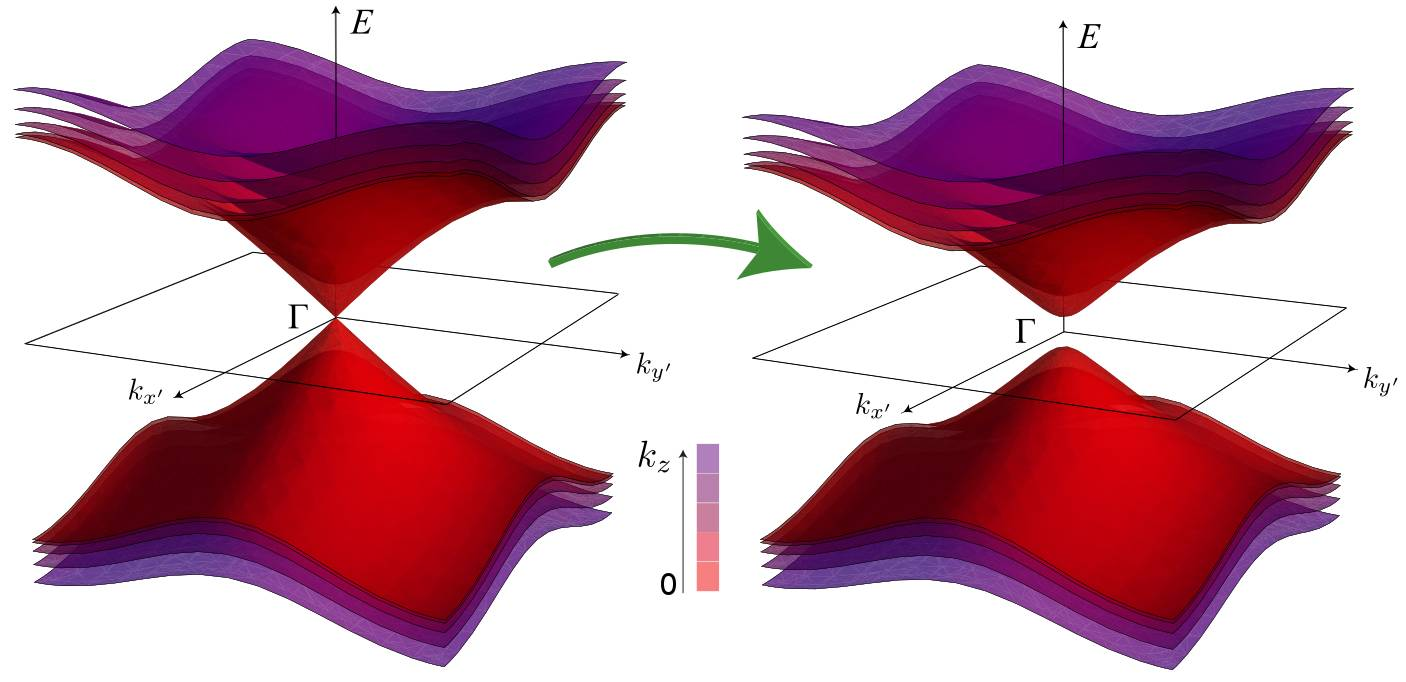
\includegraphics[width=0.48\textwidth]{Diracmassjpg.jpg}
\caption{Dirac mass gap $2|\Delta|$ introduced by AFTR and $C_2$ symmetry breaking dimerization $\Delta=\Delta_1+i\Delta_2$.}\label{fig:Diracmassjpg}
\end{figure}

Remembering that the coupled wire model \eqref{WeylTBHam} (figure~\ref{fig:WeylTB}) descended from a vortex lattice of the microscopic parent Dirac Hamiltonian \eqref{DiracHam}, the Dirac mass $m({\bf r})$ actually allows the model to carry fewer symmetries than the low-energy effective Hamiltonian \eqref{WeylTBHam} suggests. Now that the translation symmetry is lowered, the Brillouin zone is reduced (see figure~\ref{fig:DiracTB}(b)) so that the two Weyl points now coincide at the origin $\Gamma$. This recovers an unanomalous Dirac semimetallic model \eqref{DiracHam0} around $(k_{x'},k_{y'})=(0,0)$. The fourfold degenerate Dirac point is protected and pinned at $\Gamma$ due to the remaining \AFTR symmetry $\mathcal{T}_{11}$ -- which takes the role of a spinful time reversal ($\hat{T}^2=-1$) in the continuum limit -- and the $C_2$ (screw) symmetry about the $z$-axis. However, if any of these symmetries is further broken, the fourfold degeneracy of the Dirac point is not protected (c.f.~the original continuum Dirac model \eqref{DiracHam}). Figure~\ref{fig:DiracTB}(a) shows a dimerized coupled Dirac wire model that introduces a finite mass for the Dirac fermion. We label the Dirac fermion operators as $\psi_{r,s}^{\mu,\sigma}$, for $\sigma=\odot,\otimes$ the chirality, $\mu=A,B$ the new sublattice label, and $(r,s)$ label the coordinates of the unit cell according to the $45^\circ$-rotated $x',y'$-axes. \begin{align}\mathcal{H}'=&\sum_{r,s}\sum_{\mu=A,B}\hbar\tilde{v}\left({\psi_{r,s}^{\mu,\odot}}^\dagger k_z\psi_{r,s}^{\mu,\odot}-{\psi_{r,s}^{\mu,\otimes}}^\dagger k_z\psi_{r,s}^{\mu,\otimes}\right)\nonumber\\&+iu_1{\psi_{r,s}^{A,\odot}}^\dagger\psi_{r,s}^{A,\otimes}-iu'_1{\psi_{r,s}^{B,\odot}}^\dagger\psi_{r,s}^{B,\otimes}+h.c.\nonumber\\&-u_2{\psi_{r,s}^{B,\odot}}^\dagger\psi_{r,s}^{A,\otimes}+u'_2{\psi_{r,s}^{A,\odot}}^\dagger\psi_{r,s}^{B,\otimes}+h.c.\label{DiracTBHam}\\&-it_1{\psi_{r-1,s}^{A,\odot}}^\dagger\psi_{r,s}^{A,\otimes}+it'_1{\psi_{r+1,s}^{B,\odot}}^\dagger\psi_{r,s}^{B,\otimes}+h.c.\nonumber\\&+t_2{\psi_{r,s+1}^{B,\odot}}^\dagger\psi_{r,s}^{A,\otimes}-t'_2{\psi_{r,s-1}^{A,\odot}}^\dagger\psi_{r,s}^{B,\otimes}+h.c.\nonumber\end{align} For instance, the model is identical to the \AFTR and $C_2$ symmetric one in \eqref{WeylTBHam} when $t_j=t'_j=u_j=u'_j$ for $j=1,2$. However, when the symmetries are broken, these hopping parameters do not have to agree.

The Bloch band Hamiltonian after Fourier transformation is \begin{gather}H({\bf k})=\left(\begin{array}{*{20}c}\hbar\tilde{v}k_z\openone&h(k_{x'},k_{y'})\\h(k_{x'},k_{y'})^\dagger&-\hbar\tilde{v}k_z\openone\end{array}\right),\label{DiracBloch}\\h(k_{x'},k_{y'})=\left(\begin{array}{*{20}c}iu_1-it_1e^{-ik_{x'}}&u'_2-t'_2e^{-ik_{y'}}\\-u_2+t_2e^{ik_{y'}}&-iu'_1+it'_1e^{ik_{x'}}\end{array}\right)\nonumber\end{gather} where the $2\times2$ identity matrix $\openone$ and $h(k_{x'},k_{y'})$ acts on the sublattice $\mu=A,B$ degrees of freedom, and $-\pi\leq k_{x'},k_{y'}\leq\pi$ are the rotated momenta. We perturb about the Dirac fixed point by introducing the dimerizations $\Delta_j$ \begin{align}t_j=t'_j=u_j-\Delta_j=u'_j-\Delta_j\end{align} for $j=1,2$. About the $\Gamma=(0,0,0)$ point, \begin{align}H(\Gamma+\delta{\bf k})=&\hbar\tilde{v}\delta k_z\sigma_z-t_1\delta k_{x'}\sigma_x-t_2\delta k_{y'}\sigma_y\mu_x\nonumber\\&-\Delta_1\sigma_y\mu_z+\Delta_2\sigma_y\mu_y+O(\delta k^2).\label{DiracHamwire}\end{align} See figure~\ref{fig:Diracmassjpg} for its massive spectrum.

\begin{figure}[htbp]
\centering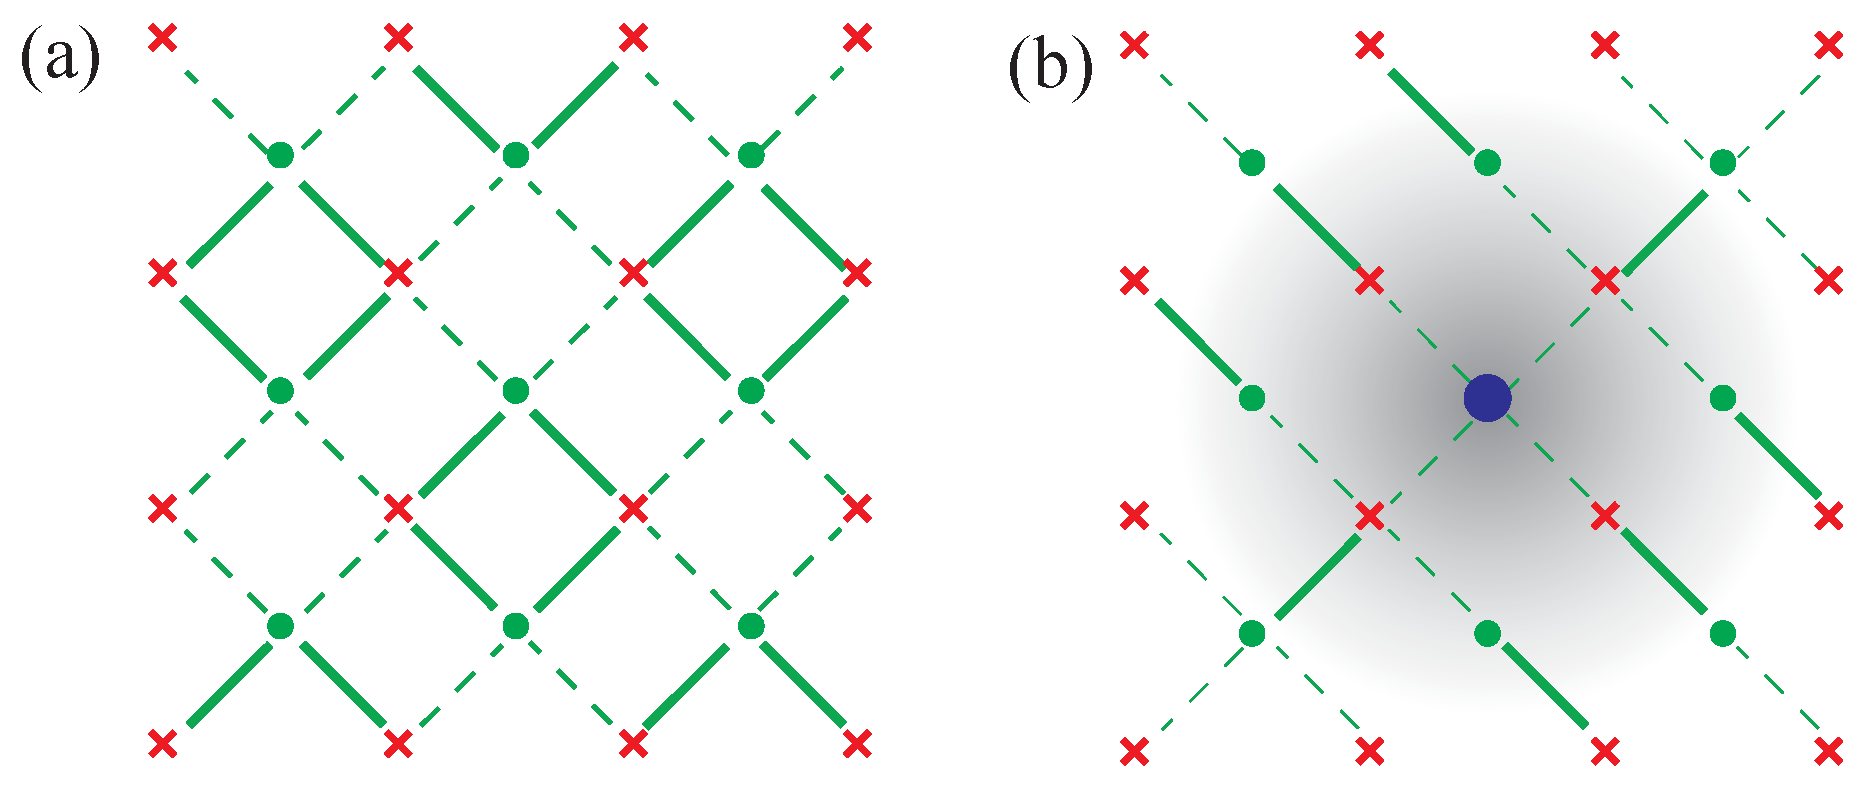
\includegraphics[width=0.4\textwidth]{dimerization}
\caption{(a) Dimerized model of a massive Dirac fermion. (b) Vortex of dimerizations $\Delta=\Delta_1+i\Delta_2$ that leaves behind a massless localized chiral Dirac channel (blue dot).}\label{fig:dimerization}
\end{figure}

Here the \AFTR symmetry $\mathcal{T}_{11}$ and the twofold rotation $\mathcal{C}_2$ are represented in the single-body picture by \begin{align}T_{11}({\bf k})&=\left(\begin{smallmatrix}0&0&-e^{ik_x}&0\\0&0&0&-1\\1&0&0&0\\0&e^{ik_x}&0&0\end{smallmatrix}\right)\mathcal{K},\nonumber\\C_2({\bf k})&=\left(\begin{smallmatrix}i&0&0&0\\0&ie^{-i(k_x+k_y)}&0&0\\0&0&-ie^{-ik_x}&0\\0&0&0&-ie^{-ik_y}\end{smallmatrix}\right)\end{align} (again suppressing the $C_2$ screw phase $e^{-ik_za/2}$ in the continuum limit $a\to0$). In the small $k_x,k_y$-limit, $T_{11}(0)=-i\sigma_y\mathcal{K}$ and $C_2(0)=i\sigma_z$. It is straightforward to check that the dimerization $\Delta_2$ preserves $\mathcal{T}_{11}$ while both $\Delta_1,\Delta_2$ breaks $C_2$.

Since the coupled wire model \eqref{DiracHamwire} and the parent continuum Dirac model \eqref{DiracHam} have the same matrix and symmetry structure, we can apply the same construction we discussed before to the new coarse-grained model \eqref{DiracHamwire}. For instance, the non-competing dimerizations $\Delta({\bf r})=\Delta_1({\bf r})+i\Delta_2({\bf r})$ can spatially modulate and form vortices in a longer length scale. Figure~\ref{fig:dimerization}(b) shows a dimerization pattern that corresponds to a single vortex in $\Delta$. The solid (dashed) lines represent strong (resp.~weak) backscattering amplitudes. In the fully dimerized limit where the dashed bonds vanish, all Dirac channels are gapped except the one at the center (showed as a blue dot). In the weakly dimerized case, there is a collective chiral Dirac channel whose wave function is a superposition of the original channels and is exponentially localized at the $\Delta$-vortex core, but now with a length scale longer than that of the original $m$-vortex lattice. These collective chiral Dirac $\Delta$-vortices can themselves form a coupled array, like \eqref{WeylTBHam}, and give a Dirac semimetal of even longer length scale. The single-body coupled vortex construction is therefore a coarse-graining procedure that recovers equivalent emergent symmetries at each step. \begin{align}\begin{diagram}\mbox{Dirac semimetal}&\pile{\rTo^{\mbox{\small mass vortices}}\\\lTo_{\mbox{\small coupled wire model}}}&\mbox{chiral Dirac strings}\end{diagram}\end{align}

\subsubsection{Holographic projection from 4D}\label{sec:holproj4D}
The coupled wire model \eqref{WeylTBHam} with two \AFTR axes can be supported by a weak topological insulator in four dimensions. Instead of realizing the chiral Dirac channels using mass vortices of a 3D Dirac semimetal, they can be generated as edge modes along the boundaries of 2D Chern insulators (or lowest Landau levels). The 4D weak topological insulator is constructed by stacking layers of Chern insulators parallel to the $zw$-plane along the $x$ and $y$ directions. The Chern layers $L_{\bf r}$, labeled by the checkerboard lattice vector ${\bf r}=r_x{\bf e}_x+r_y{\bf e}_y$ on the $xy$-plane, have alternating orientations so that $\mathrm{Ch}[L_{\bf r}]=1$ if $r_x,r_y$ are integers and $\mathrm{Ch}[L_{\bf r}]=-1$ if $r_x,r_y$ are half-integers.  The model therefore carries both \AFTR symmetries $\mathcal{T}_{11}$ and $\mathcal{T}_{\bar{1}1}$ as well as the $C_2$ rotation about $zw$, and when cleaved along a 3D hyper-surface normal to $w$, it generates the array of alternating chiral Dirac channels in figure~\ref{fig:WeylTB}.

The 4D weak topological insulator model can also be regarded as a stack of 3D antiferromagnetic topological insulators~\cite{MongEssinMoore10}. Restricting to the 3D hyperplane normal to $-{\bf e}_x+{\bf e}_y$, this model consists of alternating Chern insulating layers parallel to the $wz$-plane stacked along the ${\bf e}_x+{\bf e}_y$ direction. This 3D model describes an antiferromagnetic topologic insulator with a non-trivial $\mathbb{Z}_2$ index. For instance along the boundary surfaces normal to $w$ or $z$ that preserve the antiferromagnetic symmetry $\mathcal{T}_{11}$, the model leaves behind a 2D array of alternating chiral Dirac wires. The uniform nearest wire backscattering term $t_1$ (see \eqref{WeylTBHam}) introduces a linear dispersion along the $11$-direction and gives rise to a single massless surface Dirac cone spectrum at a time reversal invariant momenta on the boundary of the surface Brillouin zone where $\mathcal{T}_{11}^2=-1$. The 4D weak topological insulator model is identical to stacking these 3D antiferromagnetic topological insulators along the $\bar{1}1$-off-diagonal direction $-{\bf e}_x+{\bf e}_y$. A more detailed discussion on coupled wire constructions of a 4D strong and weak topological insulator can also be found in Ref.~\onlinecite{ParkTeoGilbertappearsoon}.

%A single wire with a chiral Dirac mode running through it is not allowed. Here we discuss what are the possible sources of chiral Dirac modes in our model. There are two possible sources, this three-dimensional array of chiral wires is the hypersurface of a four-dimensional Topological Insulator. The other possibility is that there are strips of Pfaffians, and each chiral Dirac mode (central charge c=1, conductance $\sigma$ = 1) is a combination of two adjacent edge modes of the Pfaffian strip (central charge c=1/2, conductance $\sigma$ = 1/2) as shown in fig.x. \textcolor{red}{insert a figure later}. Both of these cases preserve both of the TR operators $\mathcal{T}_{1 \bar{1}}$ and $\mathcal{T}_{1 {1}}$.

\subsubsection{AFTR breaking surfaces}\label{sec:fermiarcAFTRbreaking}

\begin{figure}[htbp]
\centering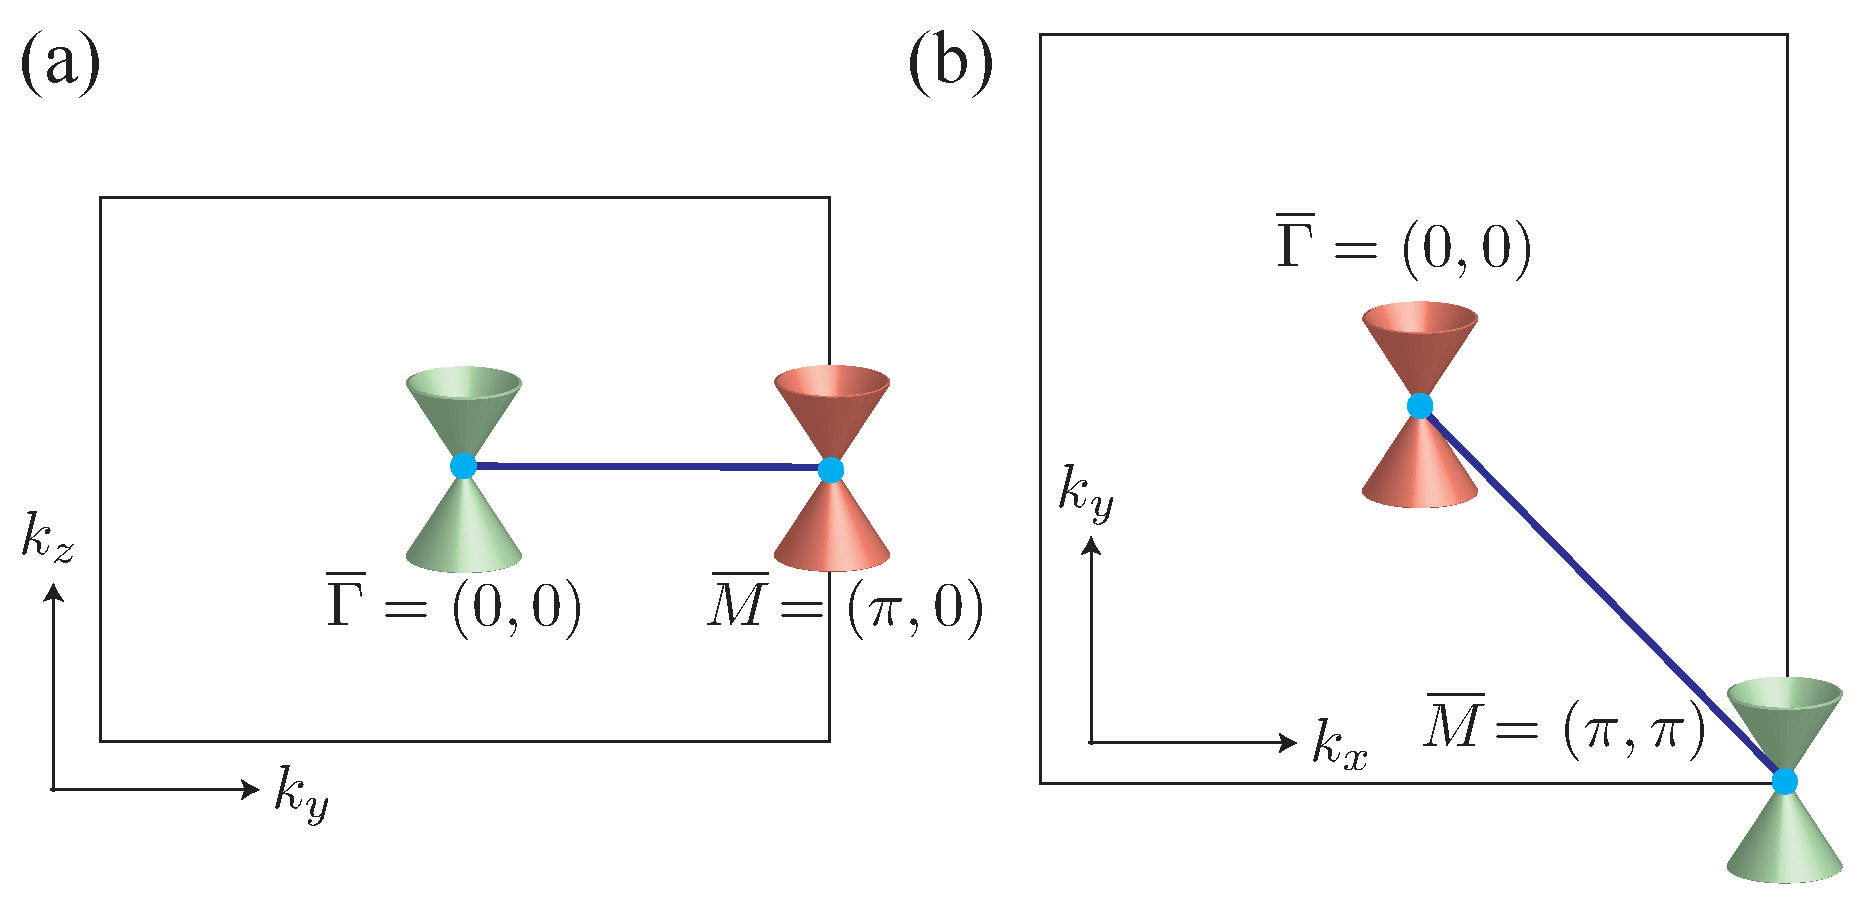
\includegraphics[width=0.4\textwidth]{fermiarc1}
\caption{Fermi arcs (blue lines) joining projected Weyl points on the surface Brillouin zones along (a) the $(100)$ surface and (b) the $(001)$ surface.}\label{fig:fermiarc1}
\end{figure}
We discuss the surface states of the coupled Dirac wire model \eqref{WeylTBHam}. Similar to the boundary surface of a translation symmetry protected Dirac semimetal (or more commonly called a Weyl semimetal), there are Fermi arcs connecting the surface-projected Weyl points~\cite{WanVishwanathSavrasovPRB11,Ashvin_Weyl_review,RMP}. First we consider the $(100)$ surface normal to $x$-axis (see figure~\ref{fig:WeylTB}). We assume the boundary cuts between unit cells and set the Fermi energy at $\varepsilon_f=0$. At $k_z=0$ and given a fixed $k_y\in(-\pi,\pi)$, the tight-binding model \eqref{BlochHam} is equivalent to the Su-Schriffer-Heeger model~\cite{SSH} or a 1D class AIII topological insulator~\cite{SchnyderRyuFurusakiLudwig08,Kitaevtable08} along the $x$-direction protected by the chiral symmetry $\sigma_zH(k_x)=-H(k_x)\sigma_z$. It is characterized by the winding number \begin{align}w(k_y)&=\frac{i}{2\pi}\int_{-\pi}^\pi \frac{1}{g(k_x,k_y)}\frac{\partial g(k_x,k_y)}{\partial k_x}dk_x\\&=\left(1+\mathrm{sgn}(k_y t_1/t_2)\right)/2.\nonumber\end{align} When $t_1,t_2$ have the same (or opposite) sign, the quasi-1D model is topological along the positive (resp.~negative) $k_y$-axis and thus carries a boundary zero mode. This corresponds to the Fermi line joining the two surface projected Weyl points at $\overline{\Gamma}$ and $\overline{M}$ (see figure~\ref{fig:fermiarc1}(a)). As the zero modes have a fixed chirality according to $\sigma_z$, they propagate uni-directionally with the dispersion $E(k_z)=\hbar\tilde{v}k_z\sigma_z$. The cleaving surface breaks \AFTR and $C_2$ symmetries, and so does the Fermi arc in figure~\ref{fig:fermiarc1}(a). For instance, any one of the \AFTR symmetries maps the boundary surface to an inequivalent one that cuts through unit cells instead of between them. As a result, the Fermi arc will connect the Weyl points along the opposite side of the $k_y$-axis for this surface. 

The $(010)$ surface Fermi arc structure is qualitatively equivalent to that of the $(100)$ surface. The $(110)$ and $(1\bar{1}0)$ surfaces that cleave along the diagonal and off-diagonal axes (see figure~\ref{fig:WeylTB}) respectively preserve the \AFTR symmetries $\mathcal{T}_{11}$ and $\mathcal{T}_{\bar{1}1}$. There are no protected surface Fermi arcs because the two bulk Weyl points project onto the same point on the surface Brillouin zone. Lastly, we consider the $(001)$ surface normal to the $z$-axis, which is the direction of the chiral Dirac strings that constitute the coupled wire model. A chiral Dirac channel cannot terminate on the boundary surface. In a single-body theory, it must bend and connect with an adjacent counter-propagating one. Although the $(001)$ plane is closed under the $C_2$ as well as both the \AFTR symmetries, the surface bending of Dirac channels must violate at least one of them. Here we consider the simplest case where the counter-propagating pair of Dirac channels within a unit cell re-connects on the boundary surface. This boundary is equivalent to a domain wall interface separating the Dirac semimetal \eqref{WeylTBHam} from an insulator where Dirac channels backscatters to their counter-propagating partner within the same unit cell. 

The domain wall Hamiltonian takes the form of a differential operator
\begin{align}\hat{\mathcal{H}}=&\sum_{m,j}-i\hbar\tilde{v}\left({\psi_{m,j}^\odot}^\dagger\partial_z\psi_{m,j}^\odot-{\psi_{m,j}^\otimes}^\dagger\partial_z\psi_{m,j}^\otimes\right)\label{WeylTBHamwall}\\&+it_1\left({\psi_{m,j}^\odot}^\dagger\psi_{m,j}^\otimes+\theta(z){\psi_{m-1,j-1}^\odot}^\dagger\psi_{m,j}^\otimes\right)+h.c.\nonumber\\&+t_2\theta(z)\left({\psi_{m-1,j}^\odot}^\dagger\psi_{m,j}^\otimes+{\psi_{m,j-1}^\odot}^\dagger\psi_{m,j}^\otimes\right)+h.c.\nonumber\end{align} by replacing $k_z\leftrightarrow-i\partial_z$ in \eqref{WeylTBHam}. Here $\theta(z)$ can be the unit step function or any function that asymptotically approaches 1 for $z\to\infty$ or 0 for $z\to-\infty$. The model therefore describes the Dirac semimetal \eqref{WeylTBHam} for positive $z$, and an insulator for negative $z$ where Dirac channels are pair annihilated within a unit-cell by $t_1$. After a Fourier transformation, the Bloch Hamiltonian $\hat{H}(k_x,k_y)$ is identical to \eqref{BlochHam} by replacing $k_z\leftrightarrow-i\partial_z$ and $g(k_x,k_y,z)=it_1(1+\theta(z)e^{-i(k_y+k_x)})+t_2\theta(z)(e^{-ik_x}+e^{-ik_y})$. Given any fixed $k_x,k_y$, the differential operator $\hat{H}(k_x,k_y)$ is identical to the Jackiw-Rebbi model~\cite{JackiwRebbi76}. Deep in the insulator, $g(k_x,k_y,z\to-\infty)=it_1$. There is an interface zero mode at the surface domain wall if $g$ changes sign, i.e.~if $g(k_x,k_y,z\to\infty)=|g|e^{i\varphi}$ has argument $\varphi=-\mathrm{sign}(t_1)\pi/2$. When $\varepsilon_f=0$, the zero modes trace out a Fermi arc that connects the two surface projected Weyl points (see figure~\ref{fig:fermiarc1}(b)).

\begin{figure}[htbp]\centering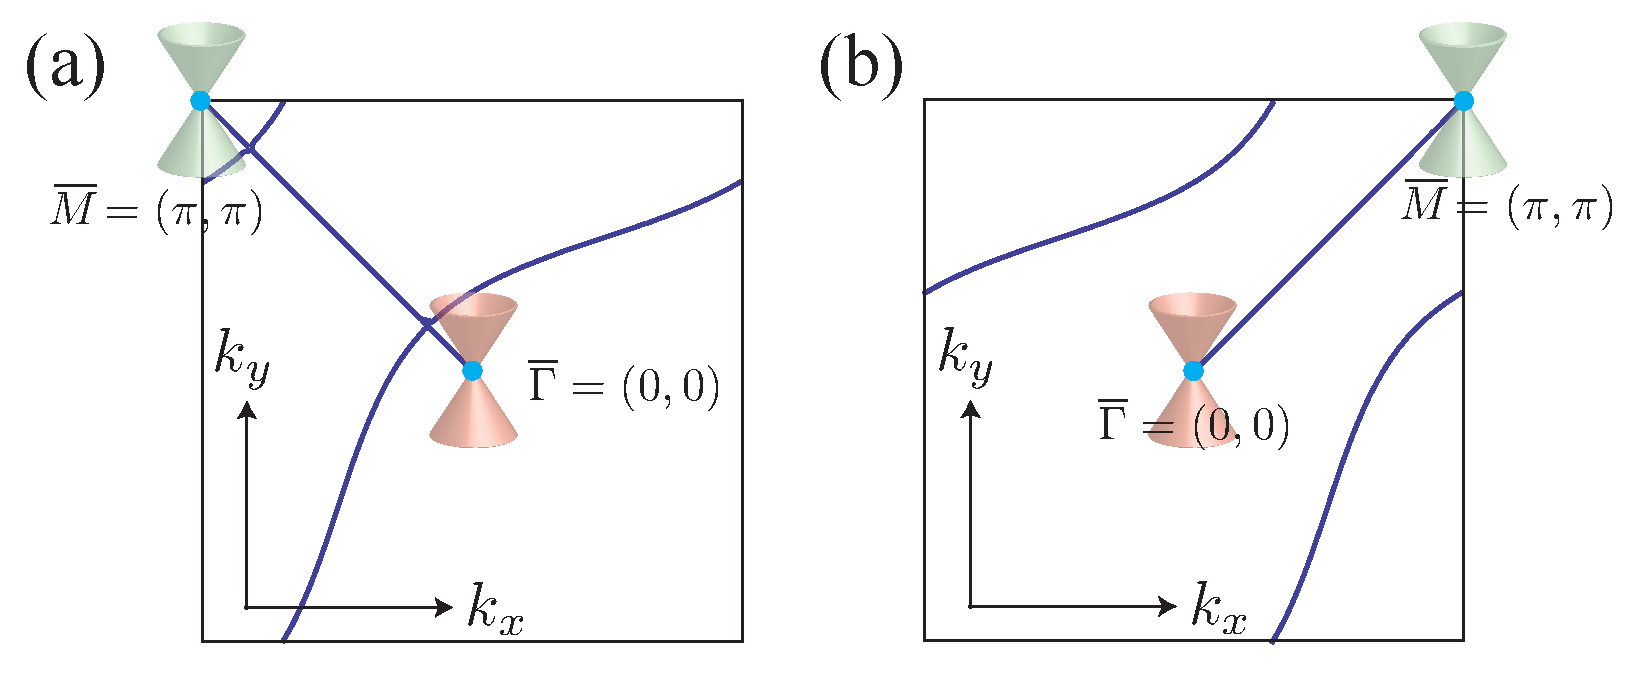
\includegraphics[width=0.4\textwidth]{fermiarc2}\caption{Fermi arcs (blue lines) on the $(001)$ surface with alternative boundary conditions (a) $g(k_x,k_y)=-it_1$ and (b) $g(k_x,k_y)=-t_2e^{-ik_y}$ in the insulating domain, for $t_2/t_1=2$.}\label{fig:fermiarc2}\end{figure}

We notice that in the insulating phase (or on the boundary surface), Dirac wires can be backscattered with a different phase and dimerized out of the unit cell. These different boundary conditions correspond to distinct surface Fermi arc patterns. Figure~\ref{fig:fermiarc2} shows two alternatives. (a) shows the the zero energy arcs when intra-cell backscattering reverses sign $t_1\to-t_1$ in the insulating domain. (b) shows a case when the dimerization is taken along the off-diagonal axis. These inequivalent boundary conditions differ by some three dimensional integer quantum Hall states, which correspond to additional chiral Fermi arcs that wrap non-trivial cycles around the 2D toric surface Brillouin zone.

\subsubsection{AFTR preserving surfaces}\label{sec:fermiarcAFTRpreserving}

We also notice that the Fermi arc structures in figures~\ref{fig:fermiarc1}(b) and \ref{fig:fermiarc2} are allowed because both the \AFTR symmetries $\mathcal{T}_{11}$, $\mathcal{T}_{\bar{1}1}$ and the $C_2$ symmetry are broken by the insulating domain. Any dimerization that preserves only one of $\mathcal{T}_{11}$ and $\mathcal{T}_{\bar{1}1}$ necessarily breaks translation symmetry, and corresponds to an enlarged unit cell and a reduced Brillouin zone (c.f.~figure~\ref{fig:Chernstack} and \ref{fig:DiracTB}). As a result, the two Weyl points would now collapse onto the same $\overline{\Gamma}$ point. Any momentum plane that contains the $k_z$-direction and avoids the $\Gamma$ point must have trivial Chern invariant, because it could always be deformed (while containing the $k_z$-direction and avoiding the $\Gamma$ point) to the reduced Brillouin zone boundary, where its Chern invariant would be killed by the \AFTR symmetry. %There would therefore be no protected surface Fermi arcs.

However, the trivial bulk Chern invariant does not imply the absence of surface state. This can be understood by looking at the surface boundary in real space. Here, we assume the Dirac strings that constitute the coupled wire model \eqref{WeylTBHam} are supported by vortices of an underlying Dirac mass (see figure~\ref{fig:vortexlattice} and eq.\eqref{DiracHam}). The semimetallic coupled wire model terminates along the $xy$-plane against vacuum, which is modeled by the Dirac insulator $H_{\mathrm{vacuum}}=\hbar v{\bf k}\cdot\vec{s}\mu_z+m_0\mu_x$, say with $m_0>0$. Recall from \eqref{massT11} that the Dirac mass vortex configuration \eqref{Jacobielliptic} is \AFTR symmetric along the $\mathcal{T}_{11}$-directions. The Dirac insulating vacuum is symmetric under local time reversal as well as continuous translation. It however breaks the screw rotation symmetry $\hat{C}_2=is_z\mu_z$, but we here only focus on the \AFTR symmetry.

\begin{figure}[htbp]
\centering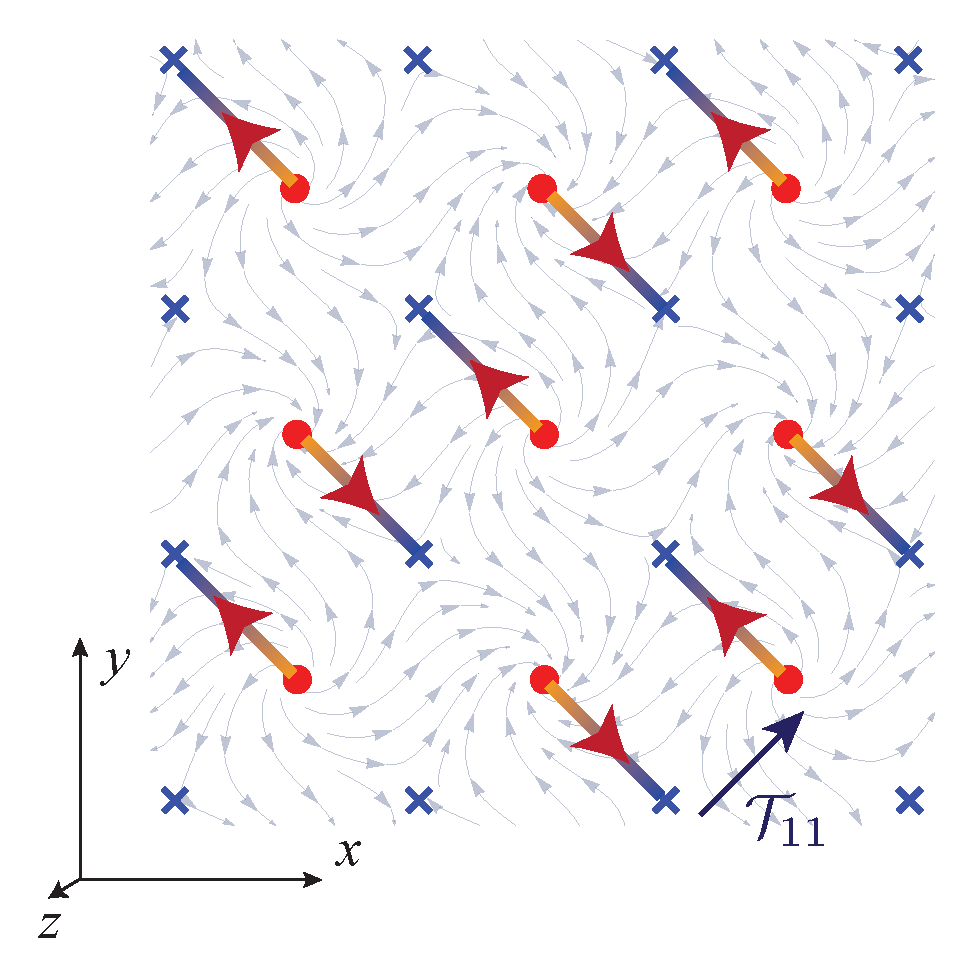
\includegraphics[width=0.3\textwidth]{SurfaceStates1bdy}
\caption{Surface chiral Dirac channels of the coupled wire model \eqref{WeylTBHam} terminated along the $xy$ plane.}\label{fig:SurfaceStates1bdy}
\end{figure}

The surface boundary supports chiral Dirac channels that connect the chiral Dirac strings in the semimetallic bulk that are normal to the surface. The surface channels are shown in figure~\ref{fig:SurfaceStates1bdy}. The {\color{blue}$\times$} ({\color{red}$\bullet$}) represent chiral vortices in the bulk that direct electrons away from (resp.~onto) the surface. The vector field represents the Dirac mass $m({\bf r})=m_x({\bf r})+im_y({\bf r})$ modulation in the semimetallic bulk near the surface. The surface Dirac line channels~\cite{TeoKane} -- shown by directed lines connecting the bulk Dirac strings {\color{blue}$\times$}, {\color{red}$\bullet$} -- are located where the time reversal symmetric Dirac mass $m_x$ changes sign across the surface boundary and the time reversal breaking Dirac mass $m_y$ flips sign across the line channels along the surface. In other words, they are traced out of points on the surface where $m_x<0$ and $m_y=0$. Each of these surface channels carries a chiral Dirac electronic mode that connects the bulk chiral Dirac vortices. They can couple through inter-channel electron tunneling, but the collective gapless surface state cannot be removed from low-energy by dimerization without breaking the \AFTR symmetry $\mathcal{T}_{11}$. %The surface state is, in a sense, half of that of a weak topological insulator (or 3D stack of quantum spin Hall layers). 